\documentclass{beamer}

\usepackage[T1]{fontenc}
\usepackage[utf8]{inputenc}
\usepackage[french]{babel}
%\usepackage{pslatex}
%\usepackage{colortbl}
%\usepackage{calc}
\usepackage{graphicx}
\usepackage{hyperref}
\usepackage{listings}

\lstset{language=bash,basicstyle=\ttfamily}

\usetheme{Warsaw}

\newcommand{\git}{\texttt{git}}

\definecolor{fondtitre}{rgb}{0.20,0.43,0.09}  % vert fonce
\definecolor{coultitre}{rgb}{0.40,0.04,0.05}  % marron
\definecolor{fondtexte}{rgb}{1,1,1}           % fond blanc
\definecolor{autre1}{RGB}{250,150,5}          % vieux mauve
\definecolor{autre2}{RGB}{235,175,235}        % horrible r
\colorlet{coultexte}{black}

\setbeamercolor{structure}{fg=coultitre, bg=fondtitre!40}
\setbeamercolor{block body}{bg=fondtexte}
\setbeamercolor{normal text}{fg=coultexte,bg=fondtexte}

\setbeamertemplate{navigation symbols}{}

\setbeamertemplate{footline}{
  \hbox{
    \hspace*{-0.06cm}

    \begin{beamercolorbox}[wd=.3\paperwidth,ht=2.25ex,dp=1ex,center]{title in head/foot}
      \usebeamerfont{author in head/foot}\insertshortauthor
      \end{beamercolorbox}

      \begin{beamercolorbox}[wd=.4\paperwidth,ht=2.25ex,dp=1ex,center]{title in head/foot}
      \usebeamerfont{title in head/foot}\insertshorttitle
      \end{beamercolorbox}

      \begin{beamercolorbox}[wd=.1\paperwidth,ht=2.25ex,dp=1ex,center]{date in head/foot}
      \usebeamerfont{date in head/foot}
    \insertframenumber{} / \inserttotalframenumber\hspace*{2ex}
    \end{beamercolorbox}

      \begin{beamercolorbox}[wd=.2\paperwidth,ht=2.25ex,dp=1ex,center]{date in head/foot}
      \usebeamerfont{date in head/foot}\insertdate
      \end{beamercolorbox}}

      \vskip0pt
}

\title[ROSE]{Gestion de versions : \git}
\author{Bertrand, Clément, Laurent, Vaibhav.}
\institute{Télécom ParisTech}
\date{4 mars 2011}

%---------------------------------------

\begin{document}

\begin{frame}
  \titlepage
\end{frame}

%------------------ Plan ---------------
\section*{Plan}
\frame{\frametitle{Plan} \small \tableofcontents}

%------------------ Slides ------------
\section{Introduction}

\subsection*{Logiciels de gestion de versions}
\begin{frame}{Logiciels de gestion de versions}
  \begin{description}
  \item[Principe :] commits, branches, différences, identification\dots
  \item[Avantages :] travail collaboratif, sauvegarde, évolution\dots
  \item[Architecture :] locale, centralisée, distribuée
  \end{description}
\end{frame}

\section{Installer et configurer \git}

\subsection*{Installation}
\begin{frame}{Installation}
  \begin{itemize}
  \item paquets \git sur debian/ubuntu
  \item éventuellement qgit/gitk, meld
  \item configuration
  \end{itemize}
\end{frame}

\subsection*{Configuration}
\begin{frame}[containsverbatim]{Configuration}
  \begin{itemize}
  \item fichier de configuration \lstinline|~/.gitconfig| ou en ligne de commande \lstinline|git config|
  \item user.name
  \item user.email
  \item core.editor
  \item merge.tool
  \end{itemize}
\end{frame}

\section{Les bases de \git}
\subsection*{Statut de fichiers}
\begin{frame}{Statut de fichiers}
  \begin{figure}
    \begin{center}
      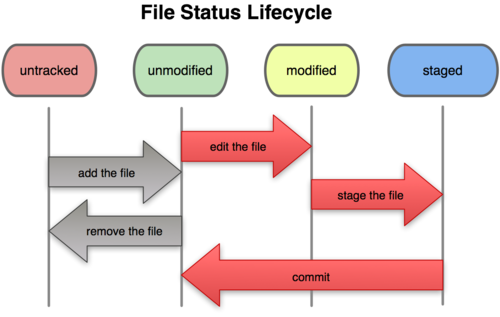
\includegraphics[scale=0.7]{img/Status_lifecycle.png}
    \end{center}
    \caption{progit.org}
  \end{figure}
\end{frame}

\subsection*{Commandes de Base}
\begin{frame}[containsverbatim]{Commandes de base}
  \begin{itemize}
  \item \lstinline|git clone| \\
    \lstinline|elecinf381@hg.comelec.enst.fr:rose2011/repo.git| \\
    - cloner un dépot distant
  \item \lstinline|git add| - ajouter un fichier ou des changements
  \item \lstinline|git rm| - supprimer un fichier ou des changements
  \item \lstinline|git status| - afficher l'état courant des fichiers
  \item \lstinline|git commit| - créer un commit avec les modifications ajoutées
  \item \lstinline|git log| - afficher l'historique
  \end{itemize}
\end{frame}

%------------------------------------------------------------
% Clément & Bertrand

\section{Gestion de branches}
\subsection*{Gestion locale}
\begin{frame}{Branches, pointeurs et commits}
  \begin{figure}
    \begin{center}
      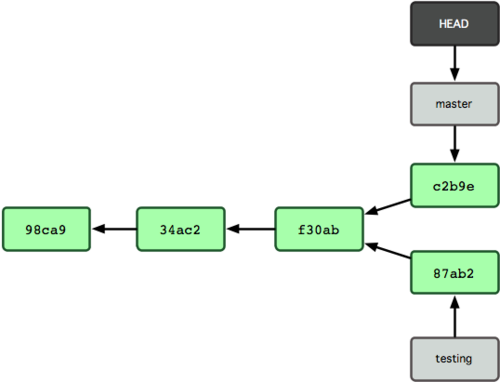
\includegraphics[scale=0.8]{img/Branch1.png}
    \end{center}
    \caption{source : progit.org}
  \end{figure}
\end{frame}

\begin{frame}[containsverbatim]{Commandes : branches}
  \begin{itemize}
  \item \lstinline|git branch| - lister les branches
  \item \lstinline|git branch <name>| - créer une branche
  \item \lstinline|git branch -d <name>| - supprimer une branche
  \item \lstinline|git checkout <branch/commit>| - se placer sur branche ou un commit
  \end{itemize}
\end{frame}

\subsection*{Interactions avec un dépot distant}
\begin{frame}{Interactions avec un dépot distant}
  \begin{itemize}
  \item \lstinline|git fetch| - se synchroniser avec le serveur
    \textbf{sans changer l'état courant}
  \item \lstinline|git push <remote> <branch>:<remotebranch>| - mettre
    à jour une branche \textbf{distante}
  \item \lstinline|git push <remote> :<remotebranch>| - supprimer une
    branche \textbf{distante}
  \end{itemize}
\end{frame}

\subsection*{Merge}
\begin{frame}{Merge 1/2}
  \begin{figure}
    \begin{center}
      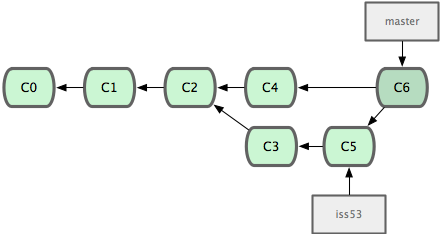
\includegraphics[scale=1]{img/Merge.png}
    \end{center}
    \caption{progit.org}
  \end{figure}
\end{frame}

\begin{frame}{Merge 2/2}
  \begin{itemize}
  \item \lstinline|git checkout <branch1>|
  \item \lstinline|git merge <branch2>|
  \item si \emph{merge conflict} :
    \begin{itemize}
    \item[] \lstinline|git status|
    \item[] \lstinline|git mergetool|
    \item[] \lstinline|git commit|
    \end{itemize}
  \item \lstinline|git pull| - fetch + merge
  \end{itemize}
\end{frame}

\section{Exemple}
\begin{frame}{}
  \begin{columns}
    \begin{column}{0.60\textwidth}
      \begin{itemize}
      \item \lstinline|git clone user@host:repo.git|
      \end{itemize}
    \end{column}
    \begin{column}{0.40\textwidth}
      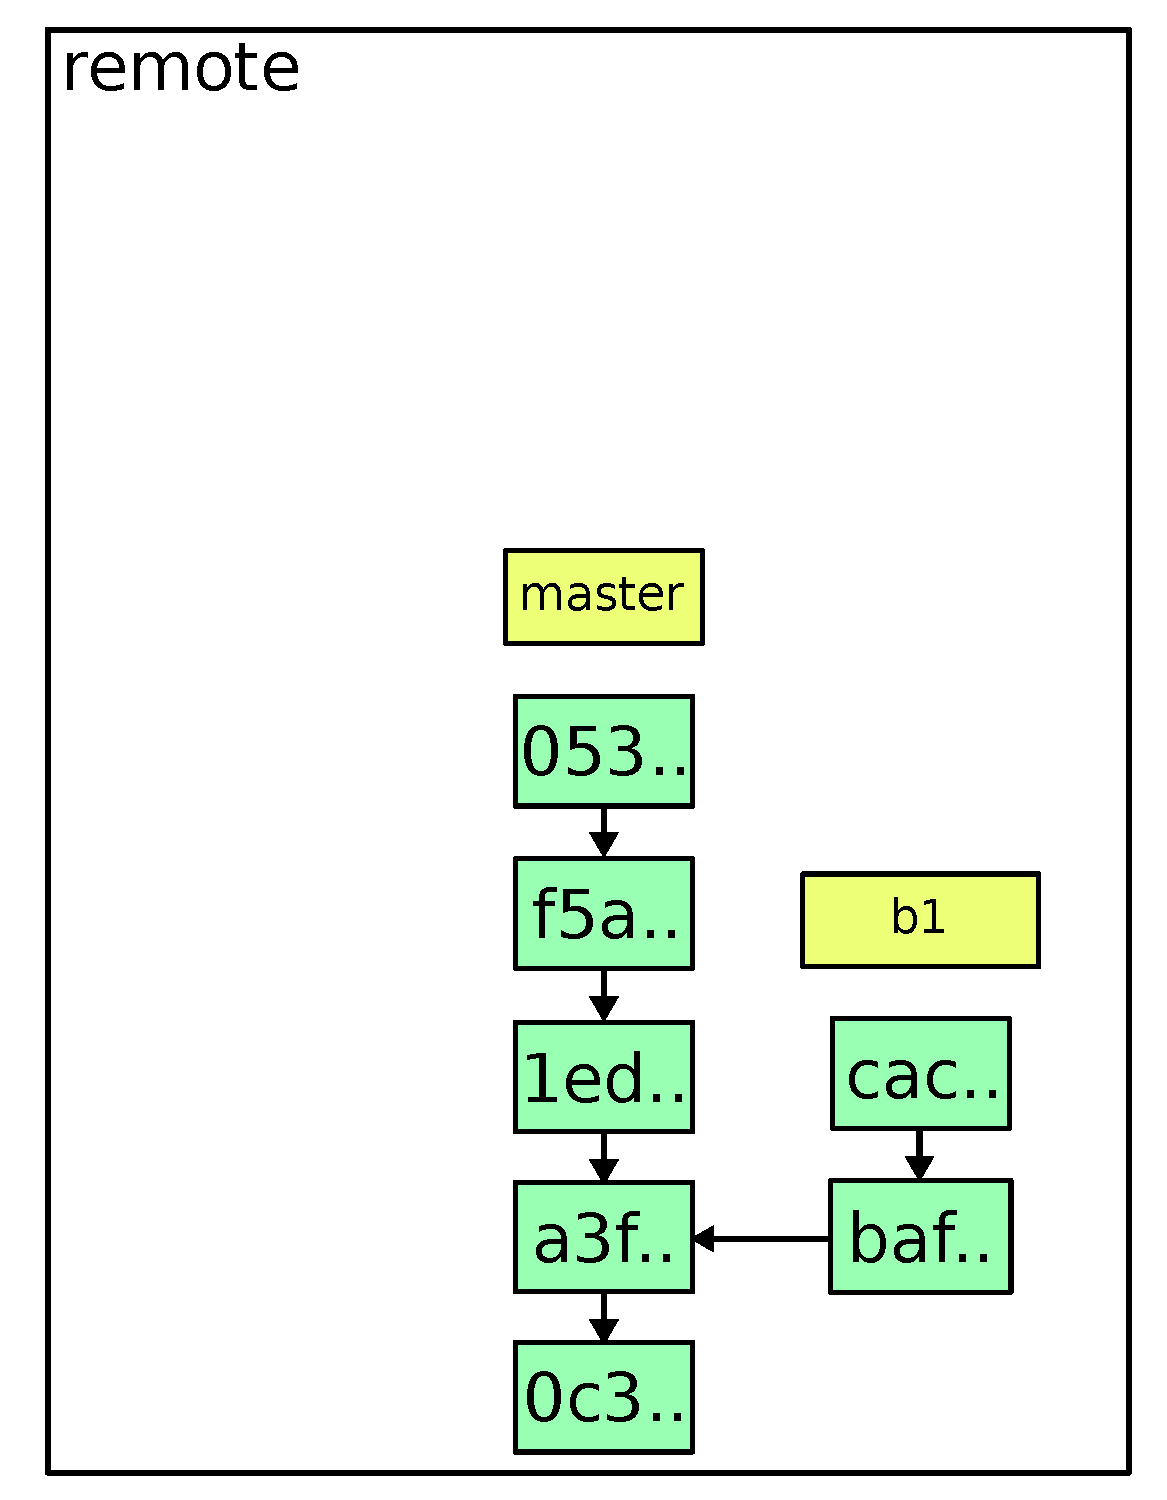
\includegraphics[width=\textwidth]{img/1.pdf}
    \end{column}
  \end{columns}
\end{frame}

\begin{frame}{}
  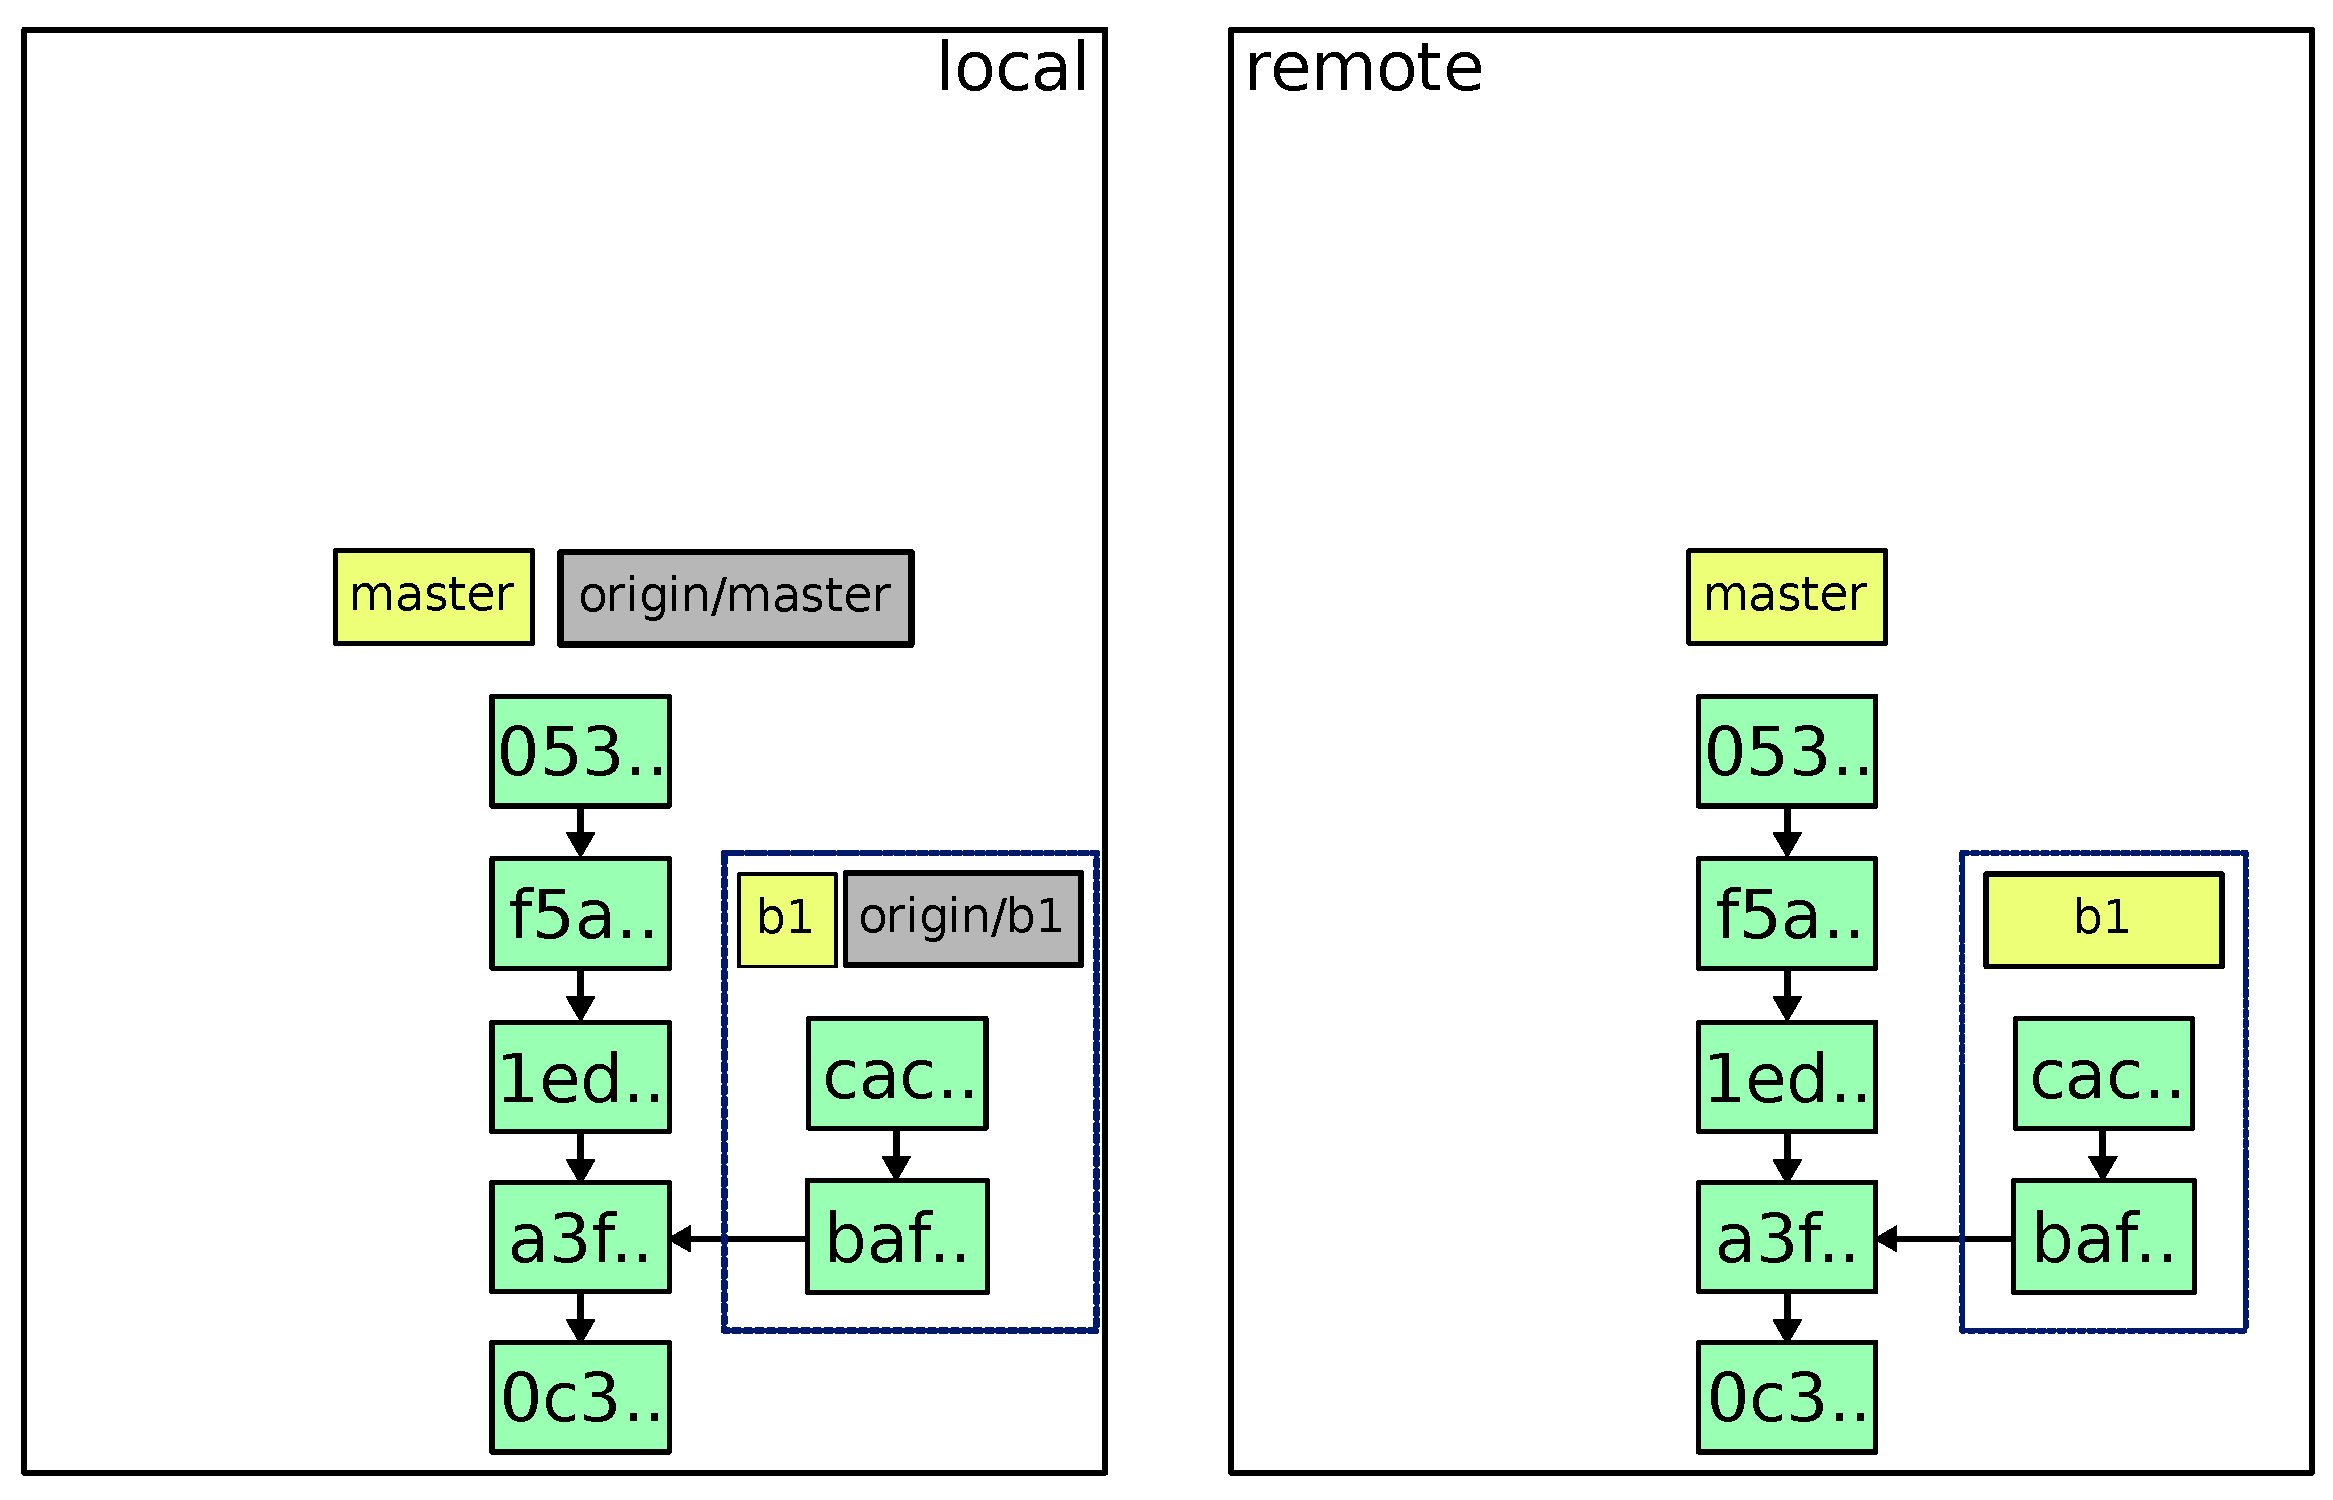
\includegraphics[width=\textwidth]{img/2.pdf}
\end{frame}

\begin{frame}{}
  \begin{itemize}
  \item \lstinline|git checkout master|
  \item \lstinline|git branch b2|
  \item \lstinline|git checkout b2|
  \end{itemize}
\end{frame}

\begin{frame}{}
  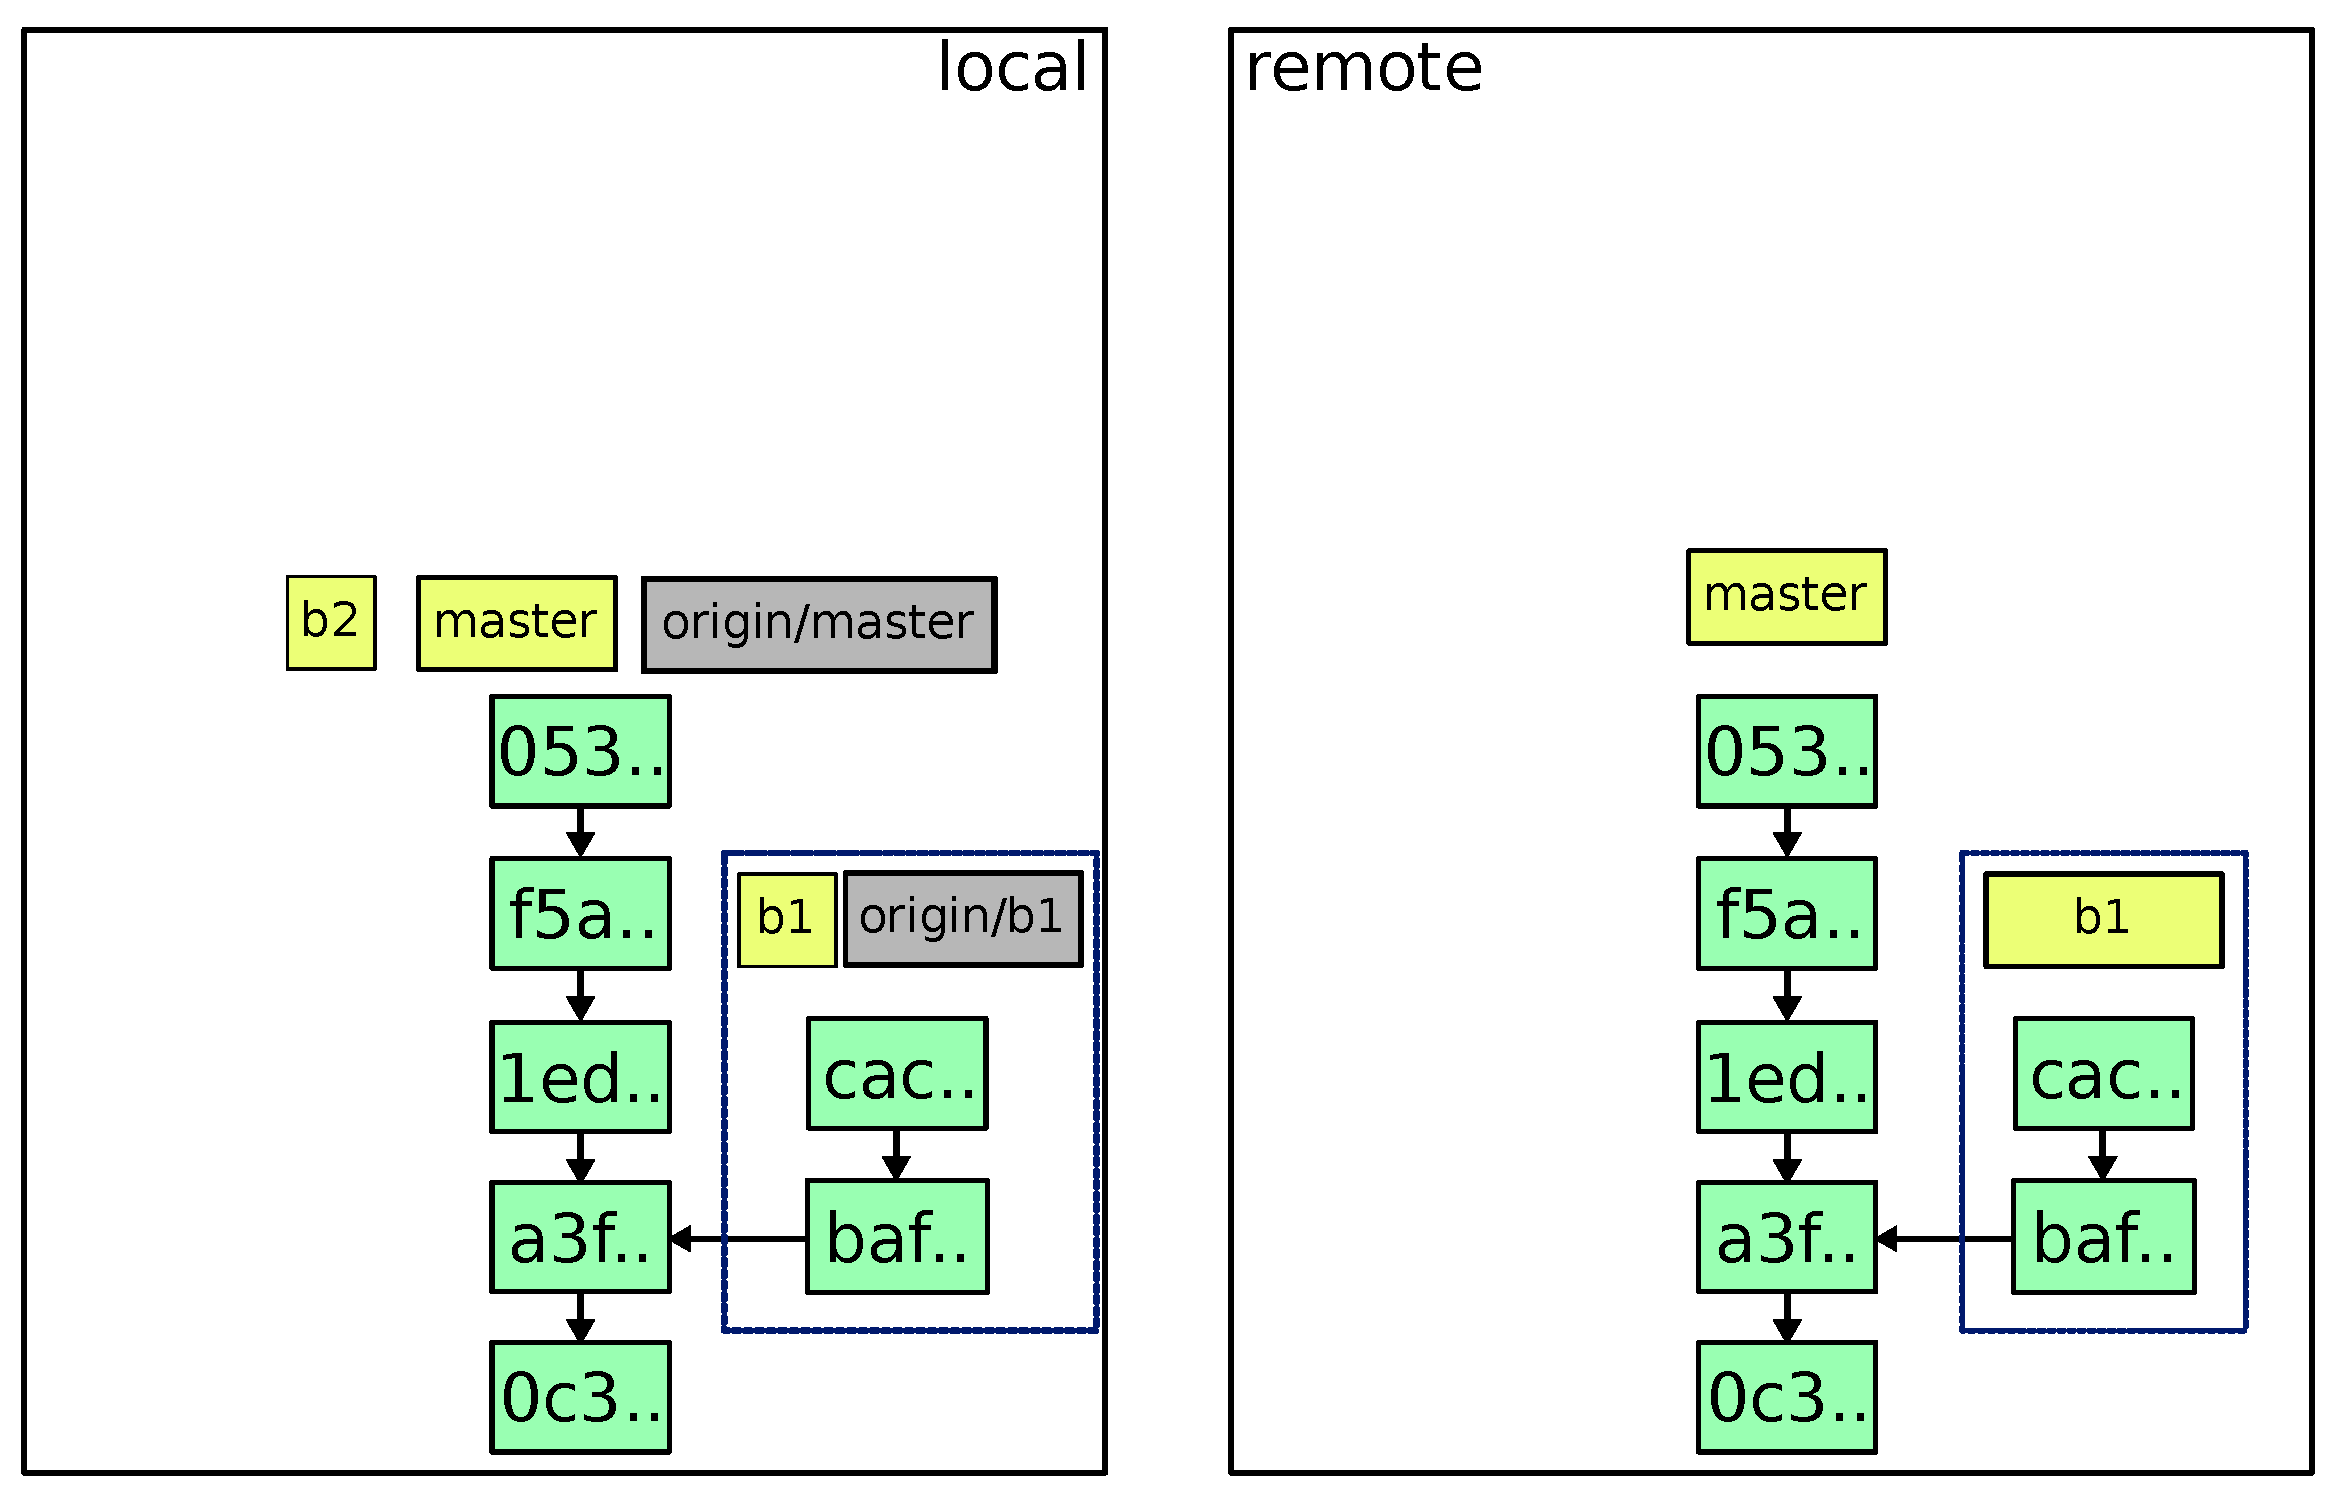
\includegraphics[width=\textwidth]{img/3.pdf}
\end{frame}

\begin{frame}{}
  \begin{itemize}
  \item faire changements
  \item \lstinline|git add <files>|
  \item \lstinline|git commit|
  \end{itemize}
\end{frame}

\begin{frame}{}
  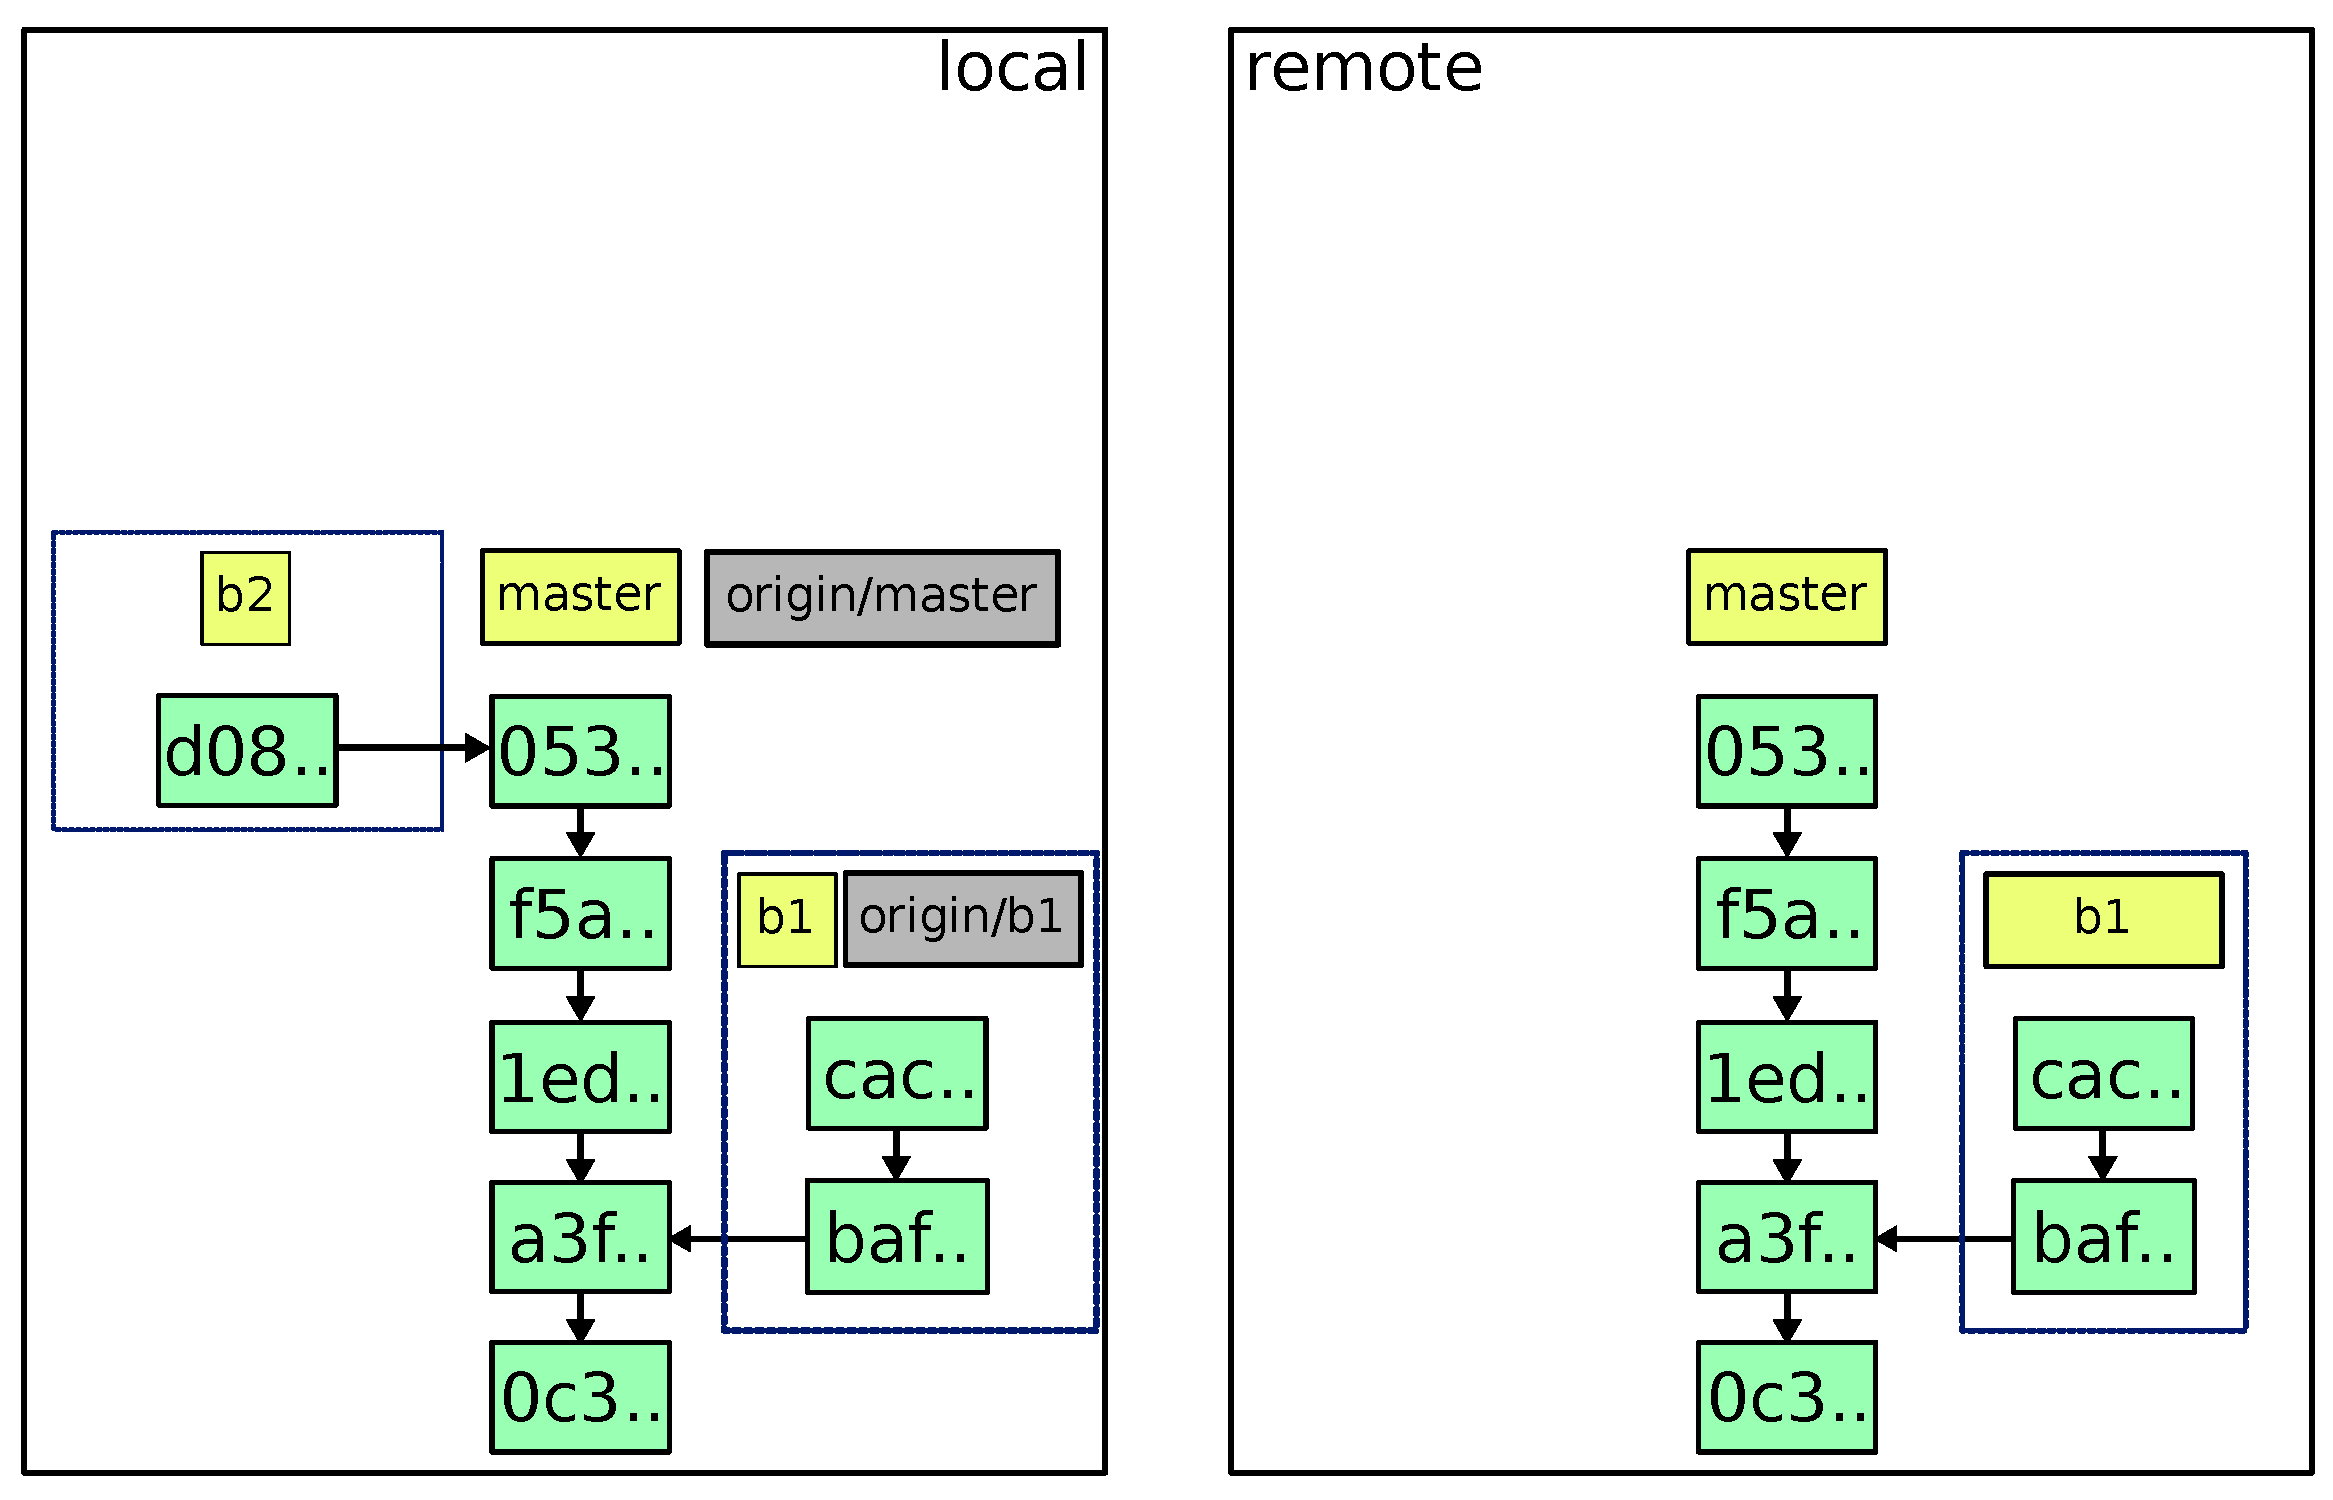
\includegraphics[width=\textwidth]{img/3-bis.pdf}
\end{frame}

\begin{frame}{}
  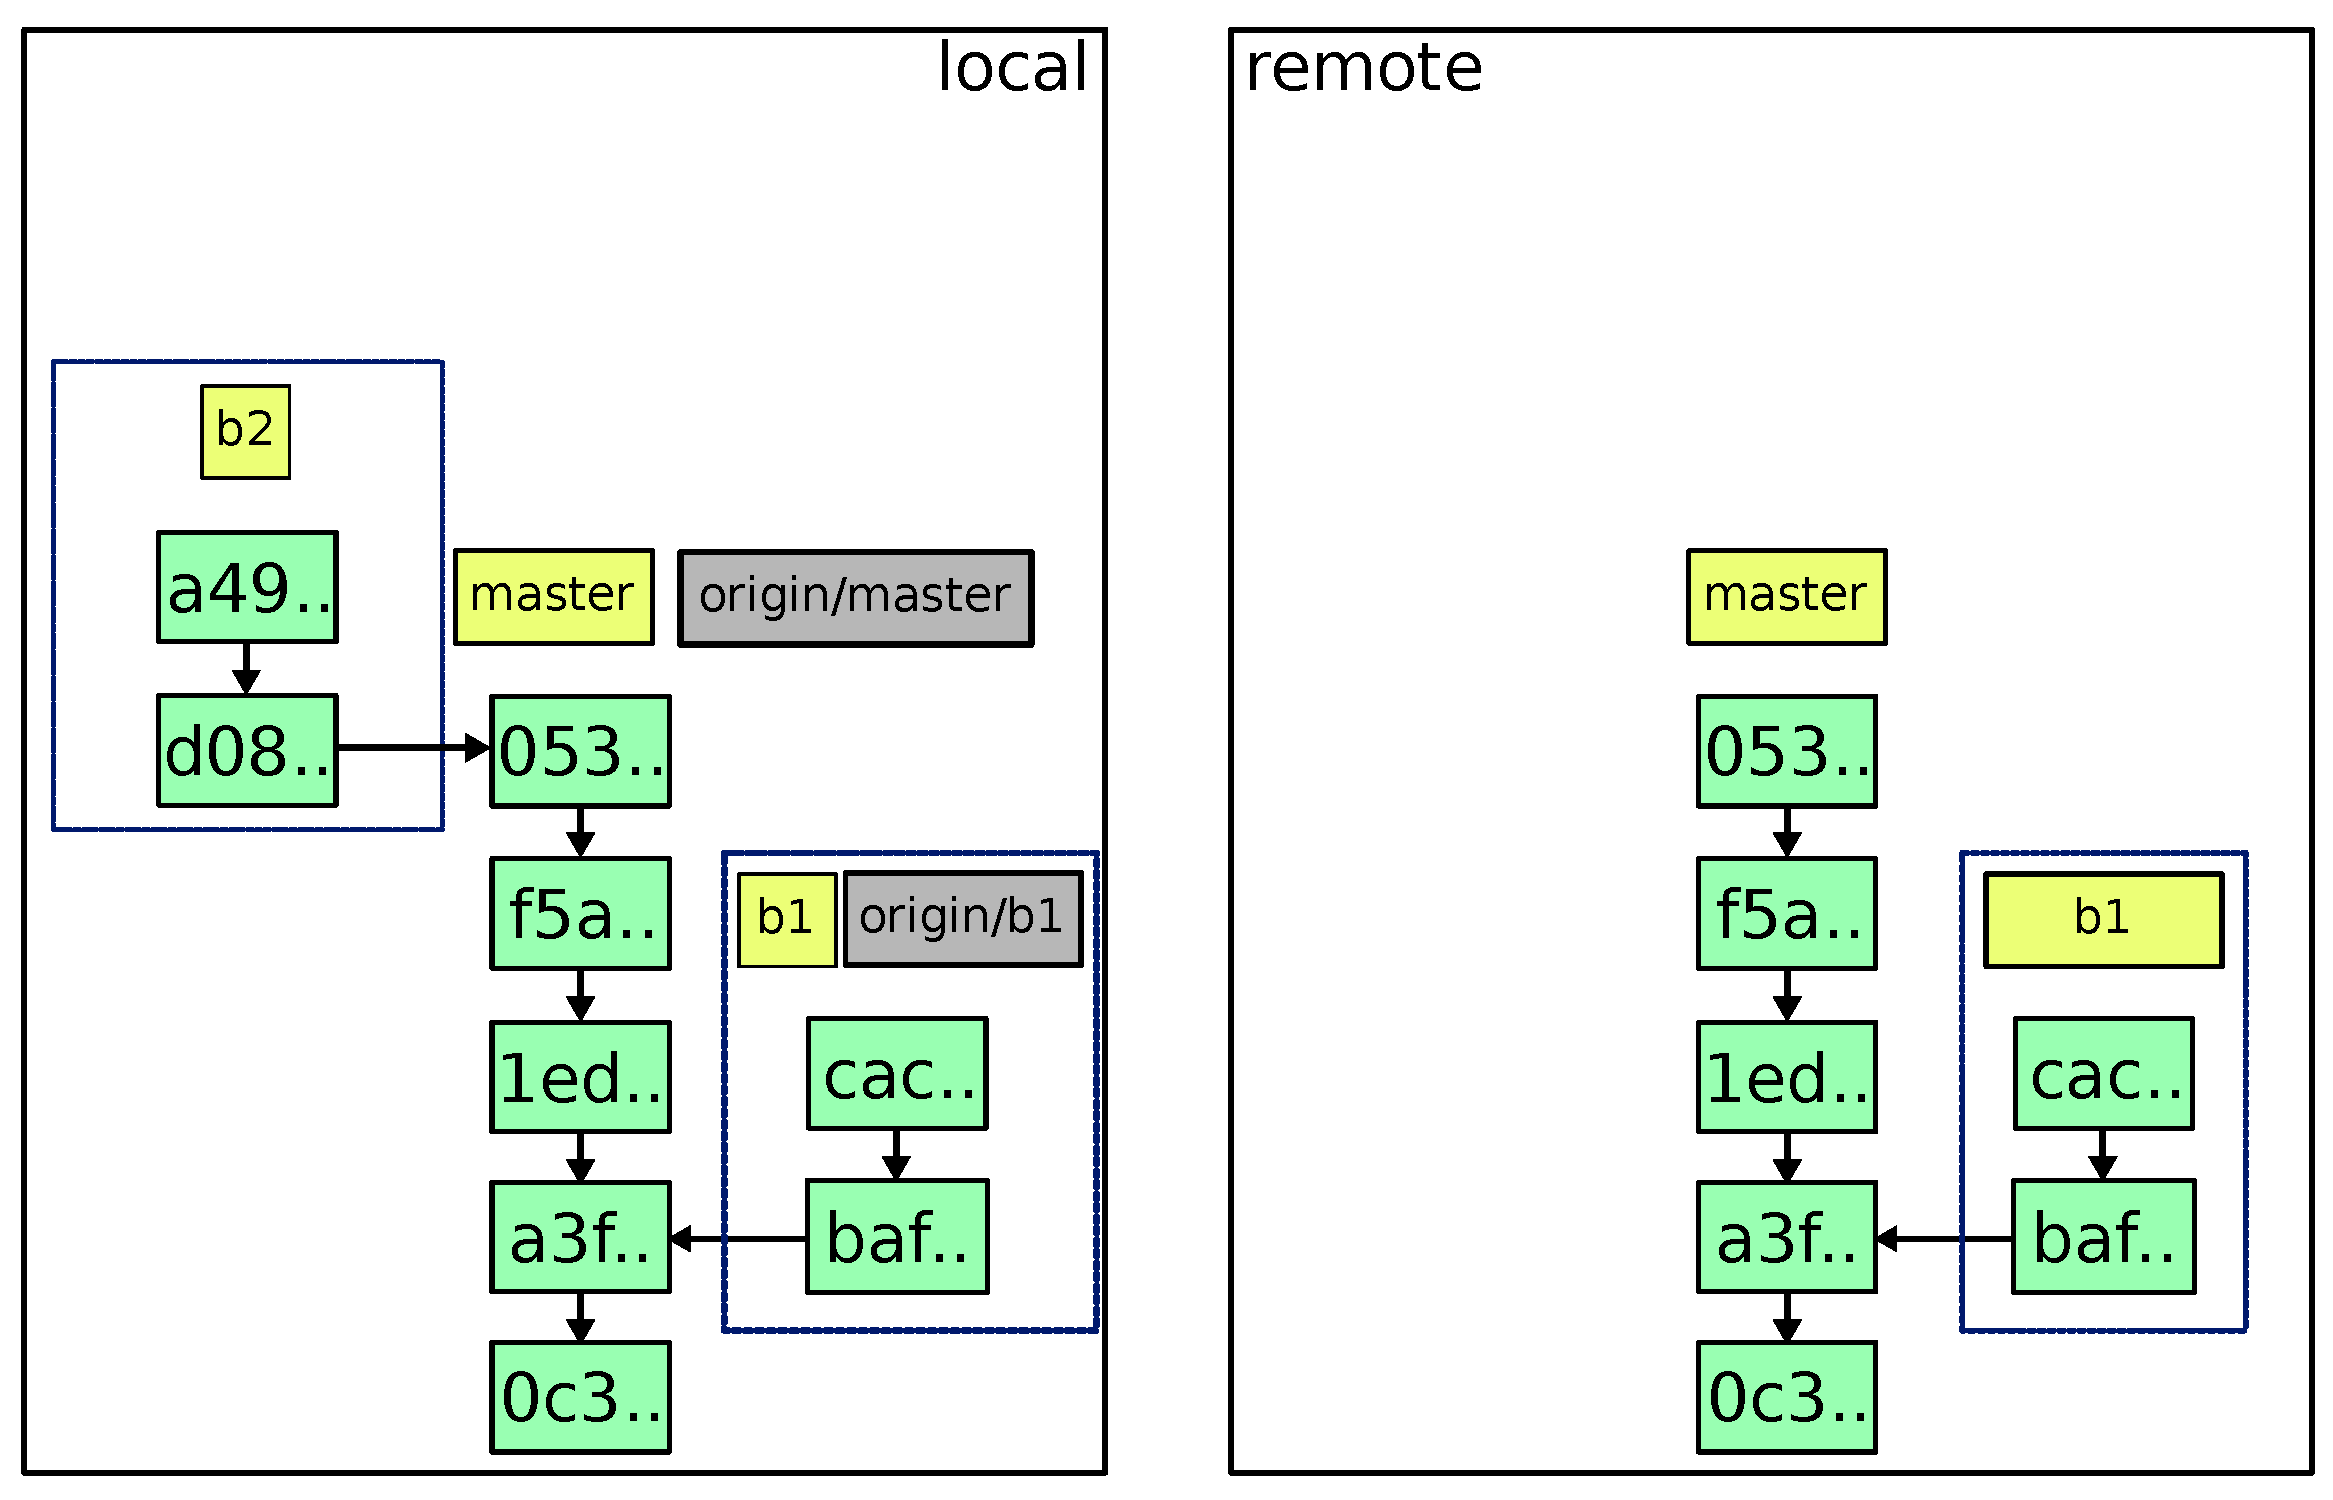
\includegraphics[width=\textwidth]{img/3-ter.pdf}
\end{frame}

\begin{frame}{}
  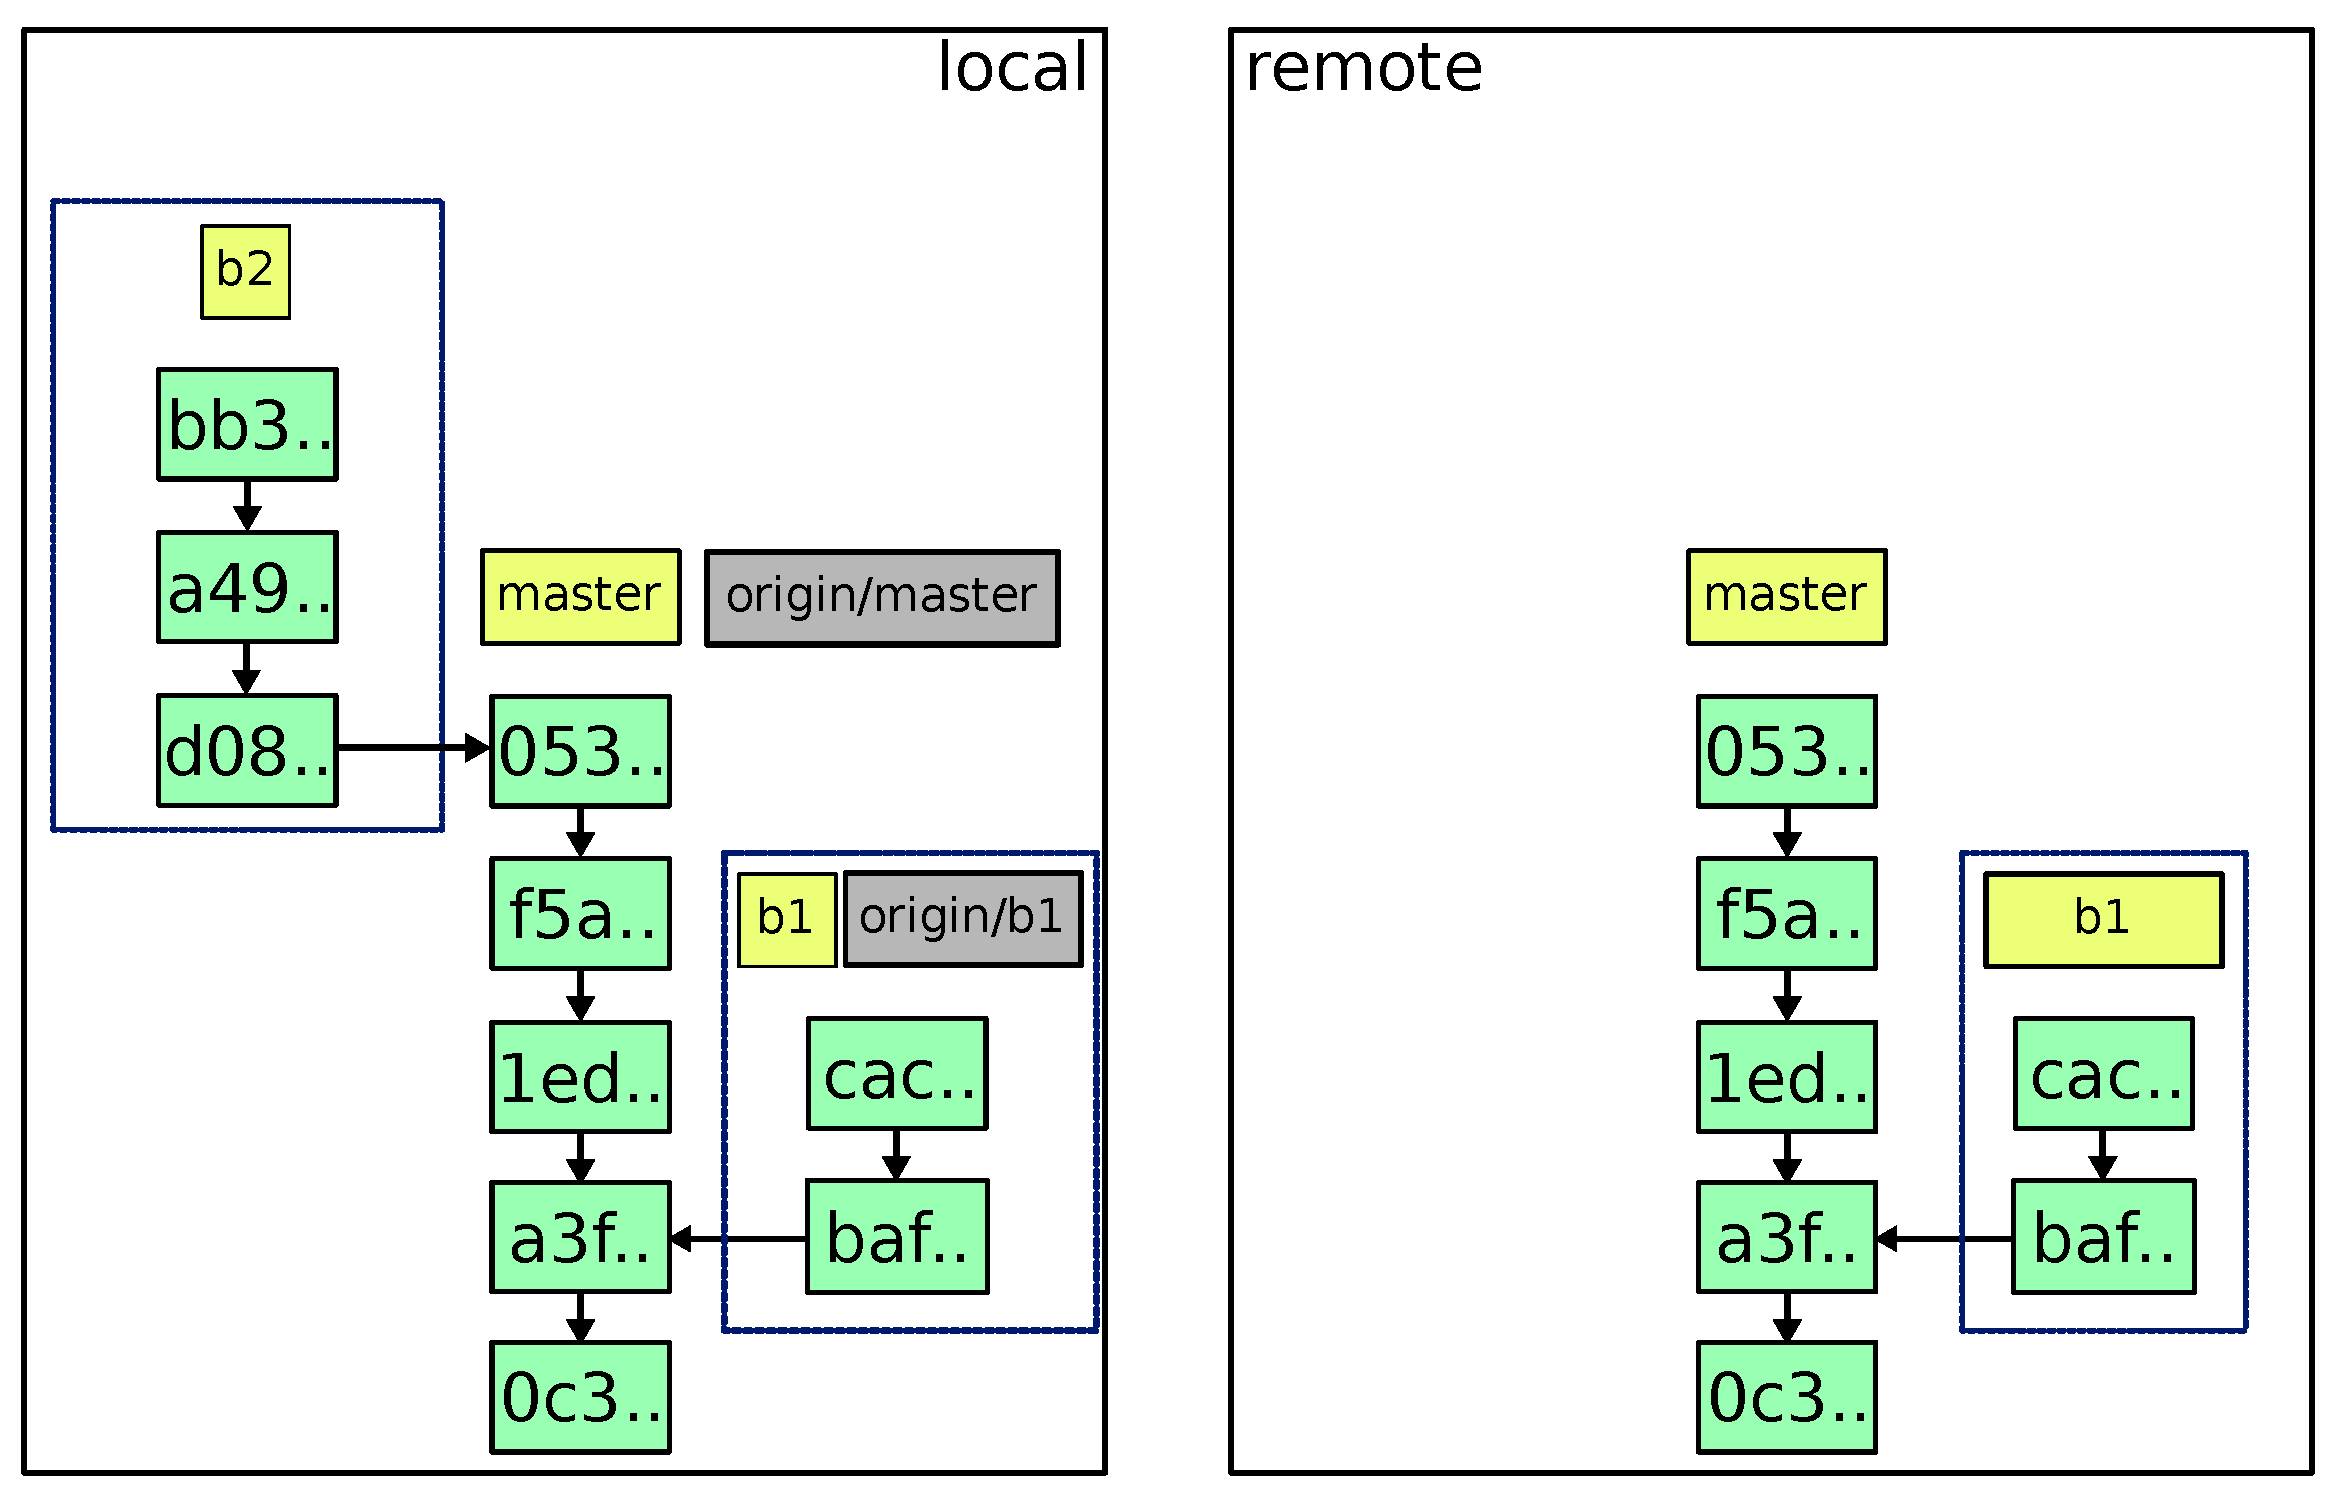
\includegraphics[width=\textwidth]{img/3-quad.pdf}
\end{frame}

\begin{frame}{}
  \begin{itemize}
  \item \lstinline|git push origin b2|
  \end{itemize}
\end{frame}

\begin{frame}{}
  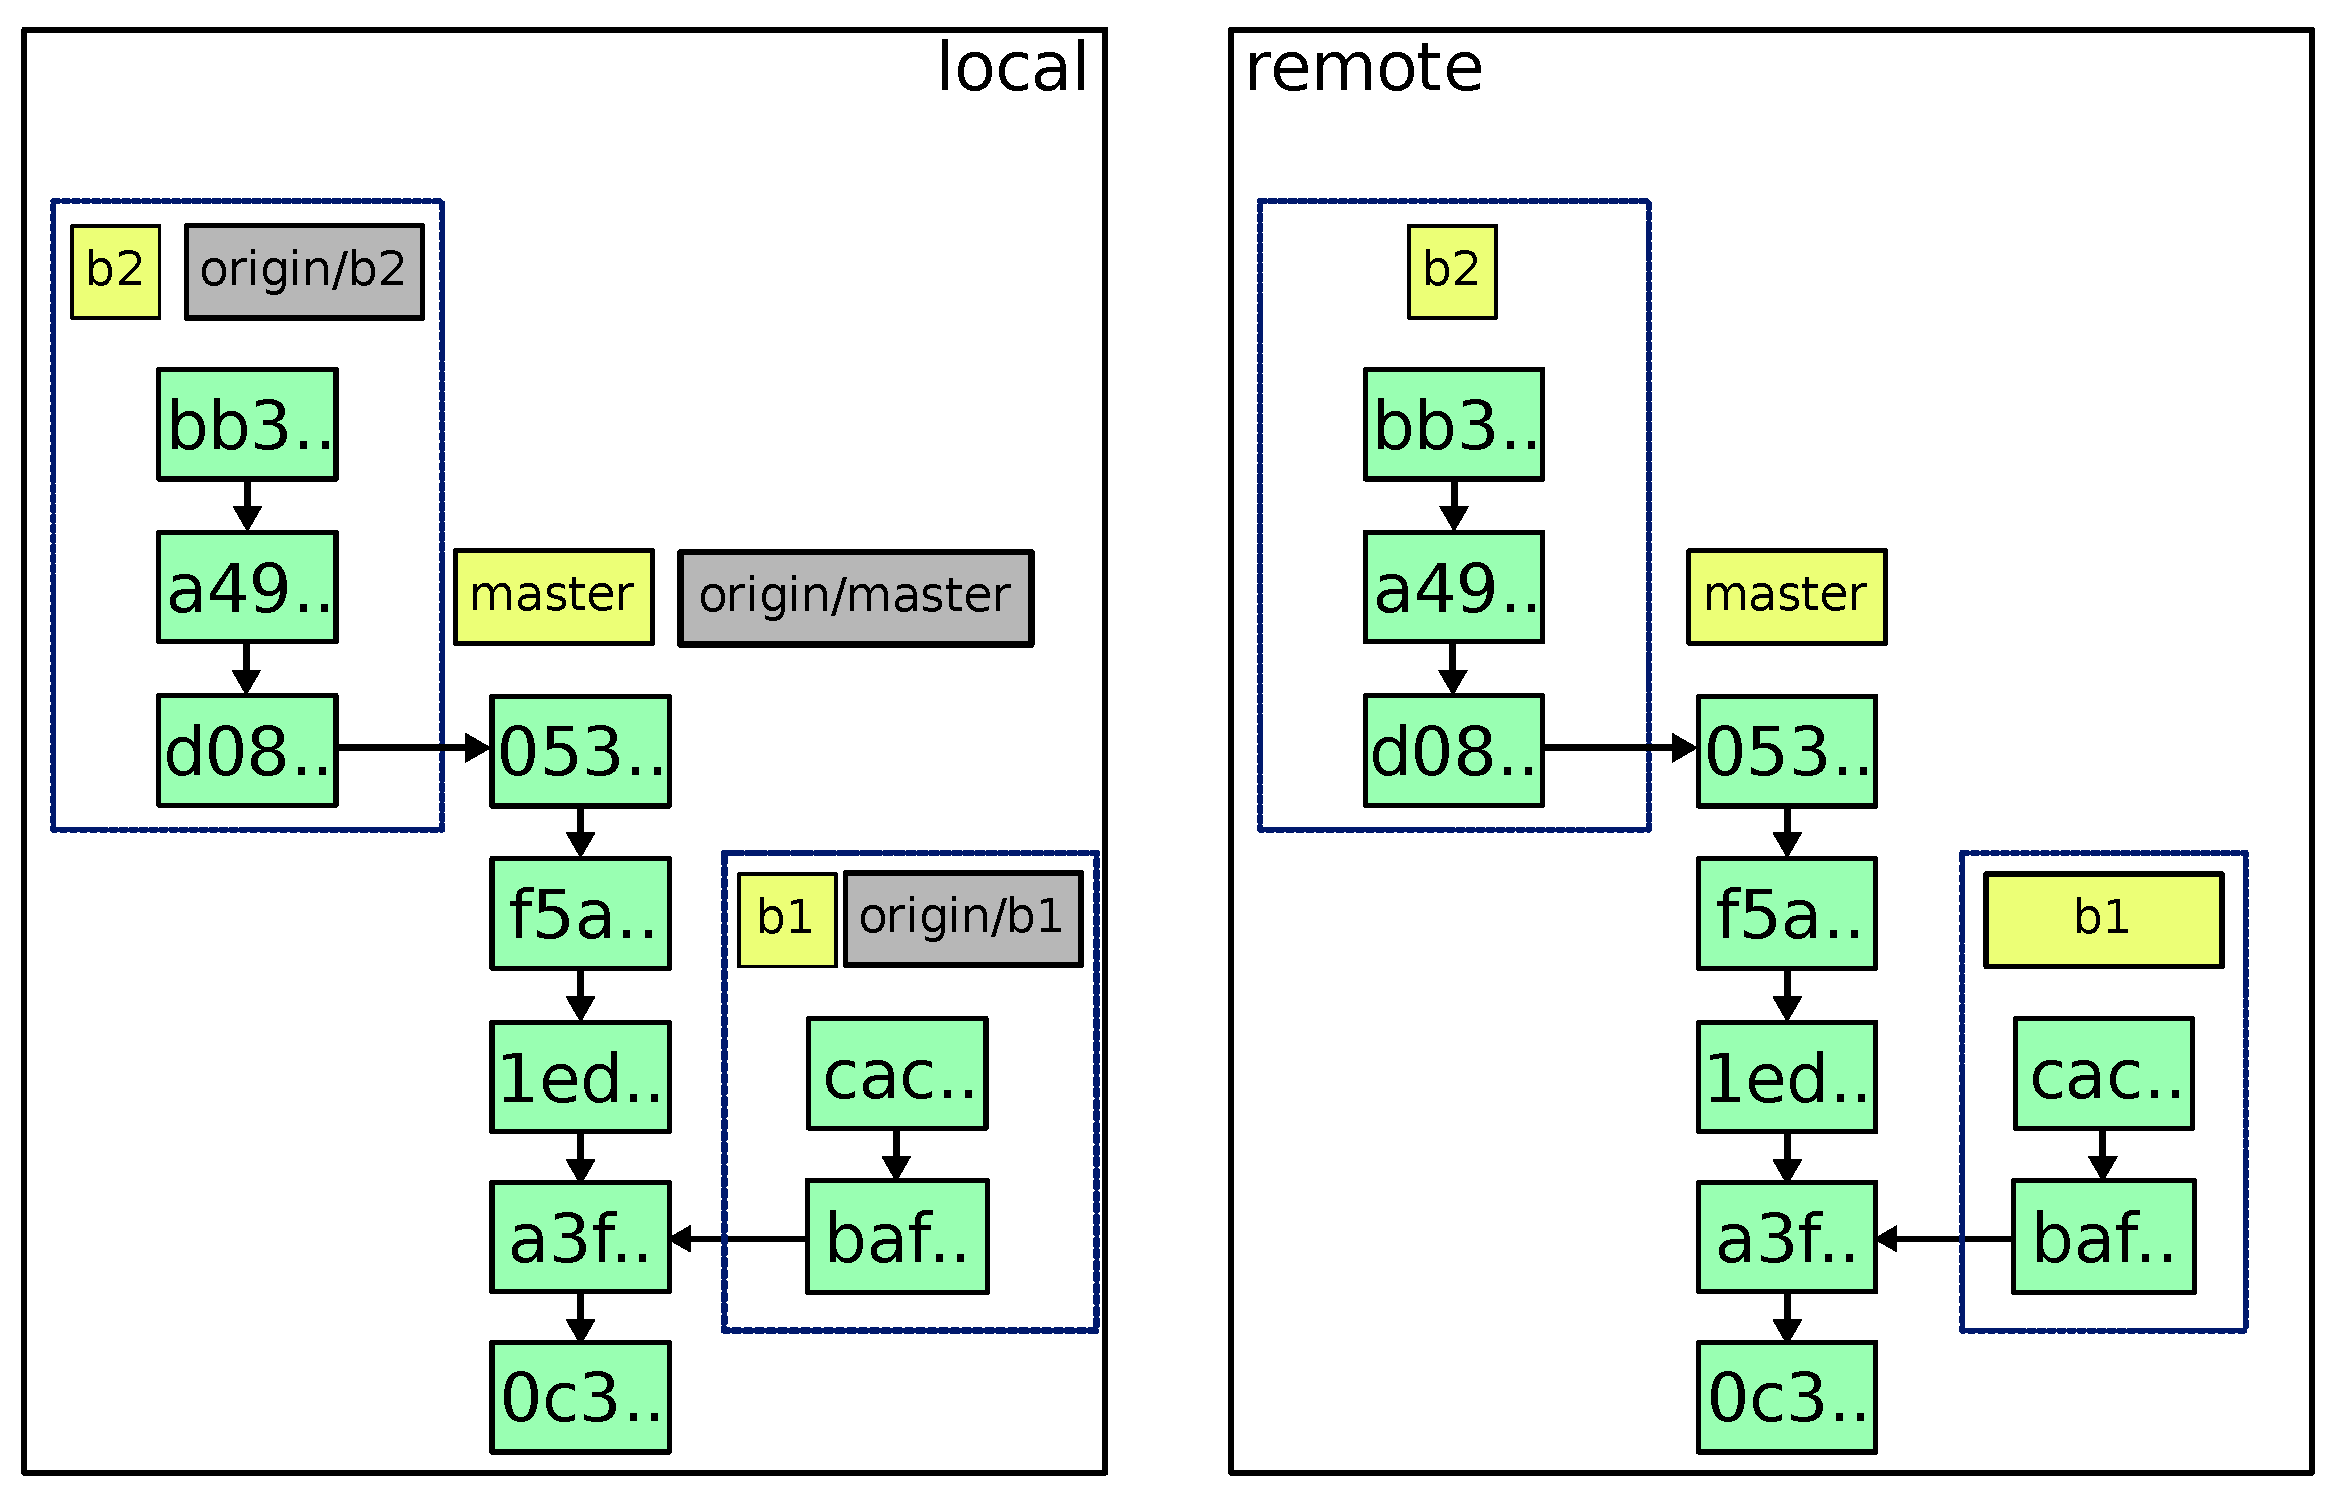
\includegraphics[width=\textwidth]{img/4.pdf}
\end{frame}

\begin{frame}{}
  \begin{itemize}
  \item \lstinline|git rebase master b1|
  \end{itemize}
\end{frame}

\begin{frame}{}
  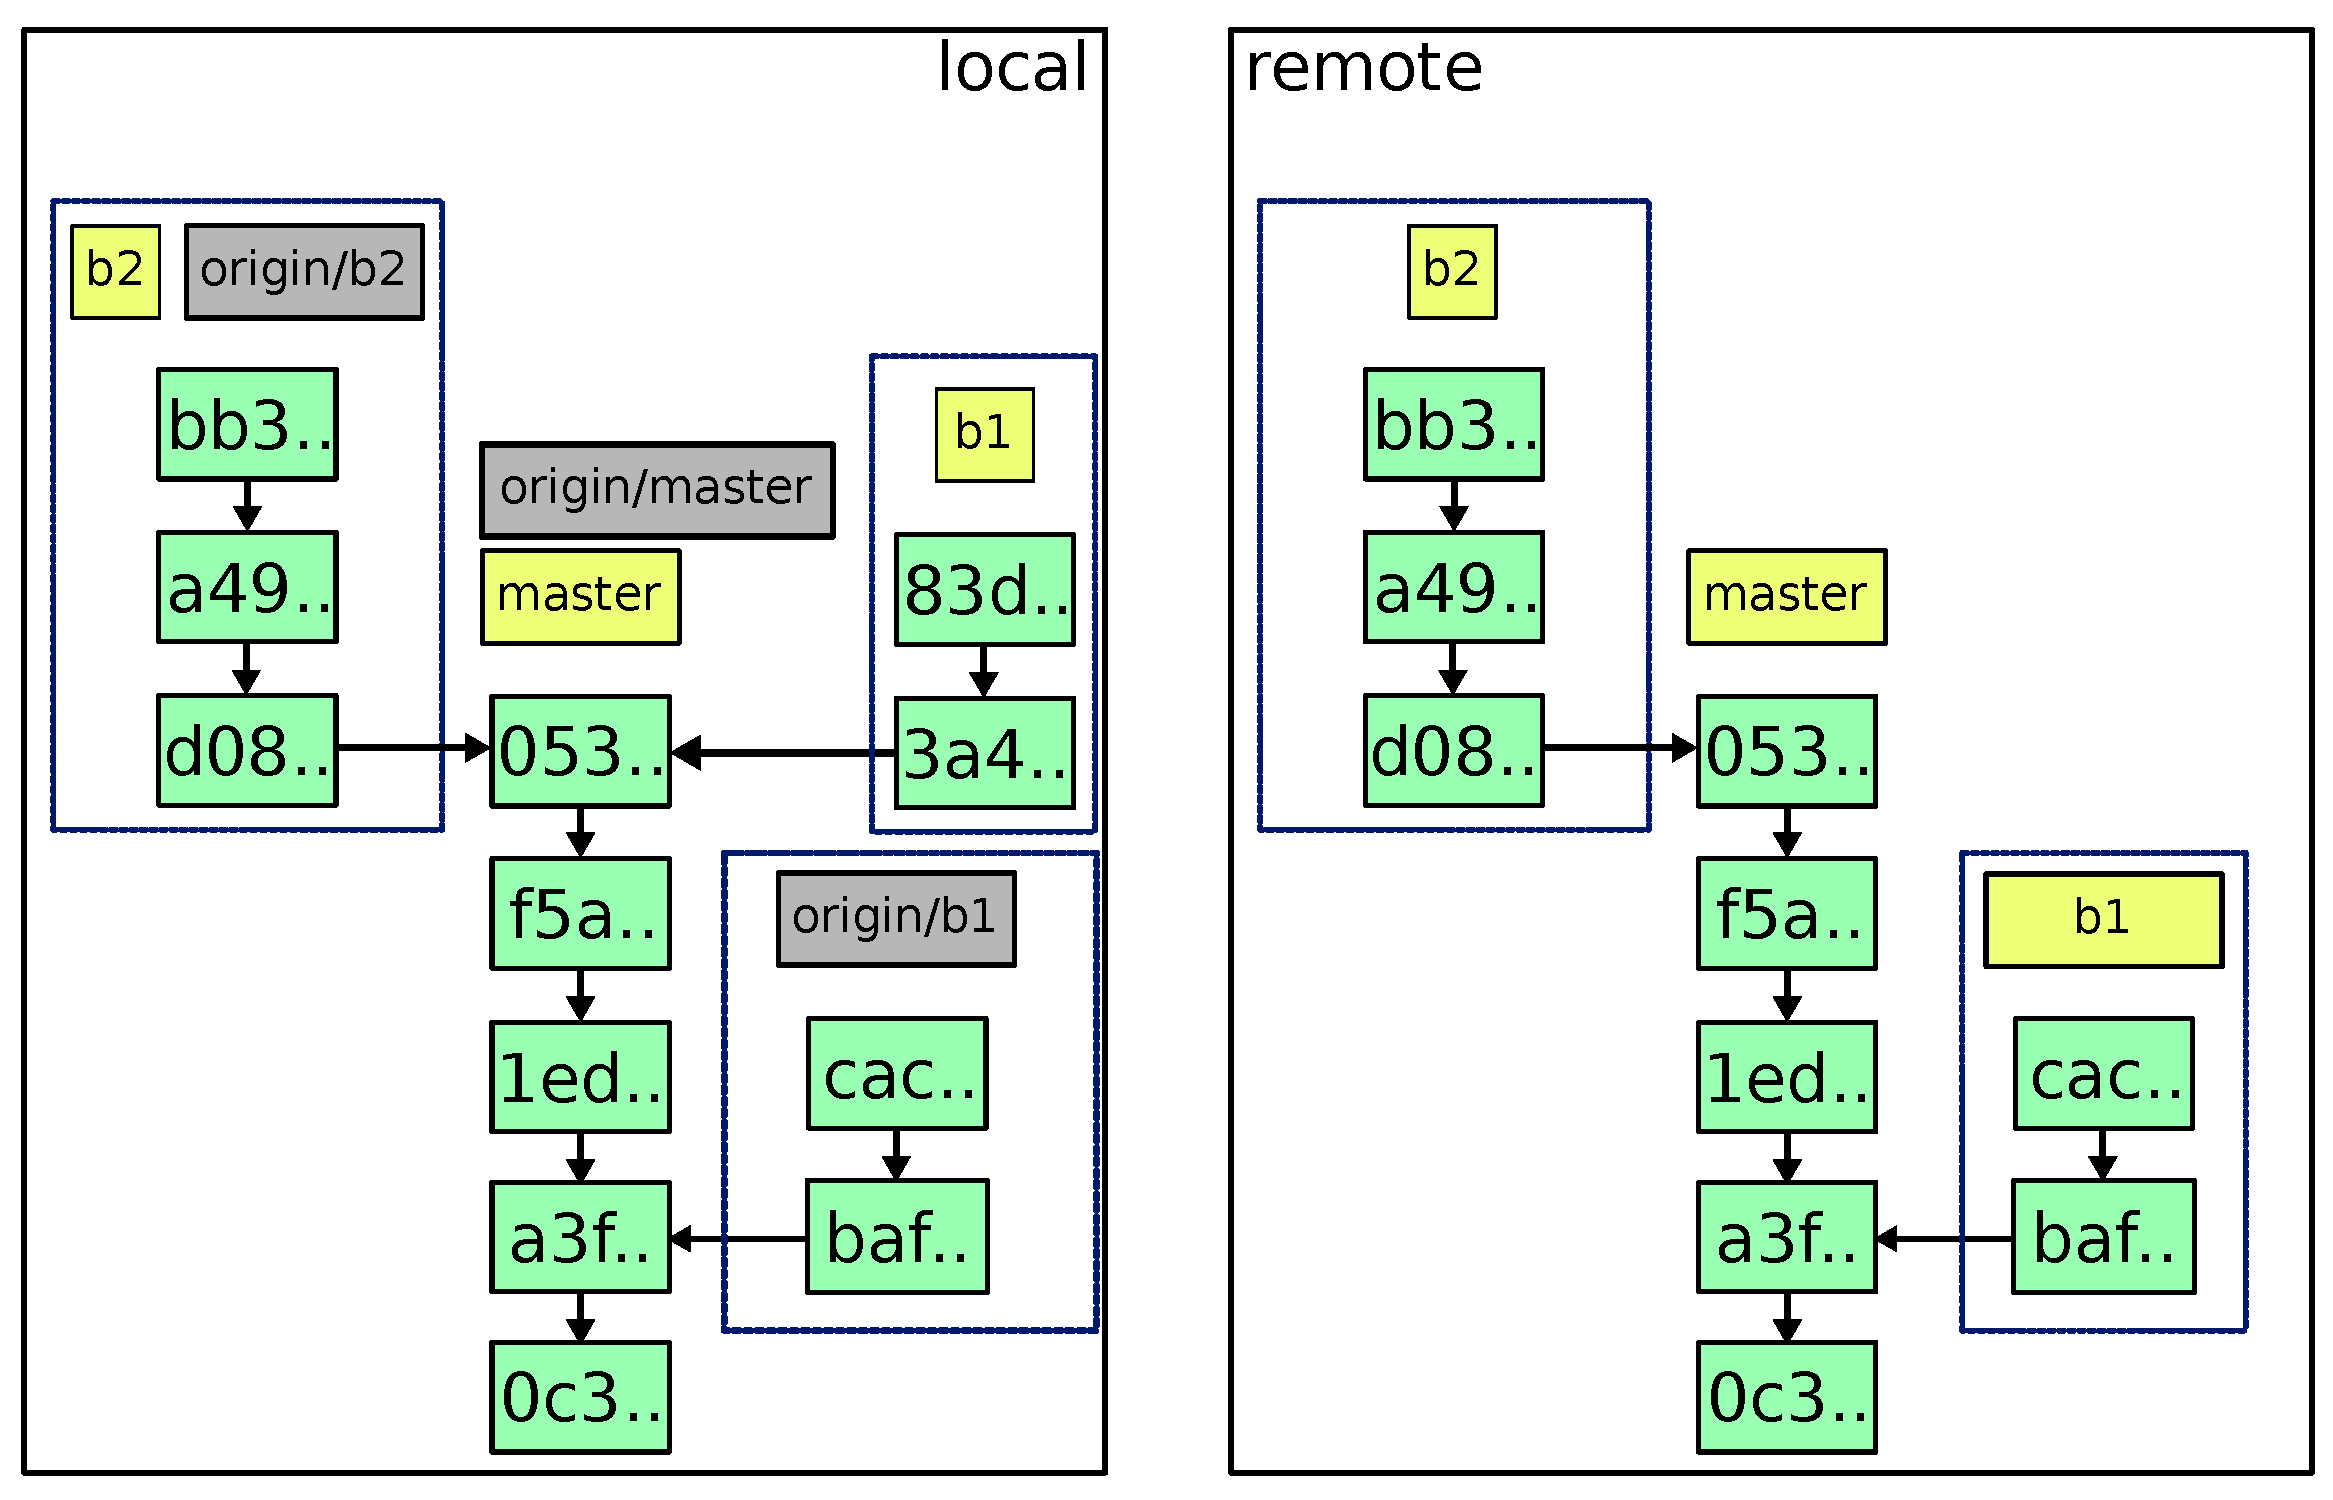
\includegraphics[width=\textwidth]{img/5.pdf}
\end{frame}

\begin{frame}{}
  \begin{itemize}
  \item \lstinline|git push -f origin b1|
  \end{itemize}
\end{frame}

\begin{frame}{}
  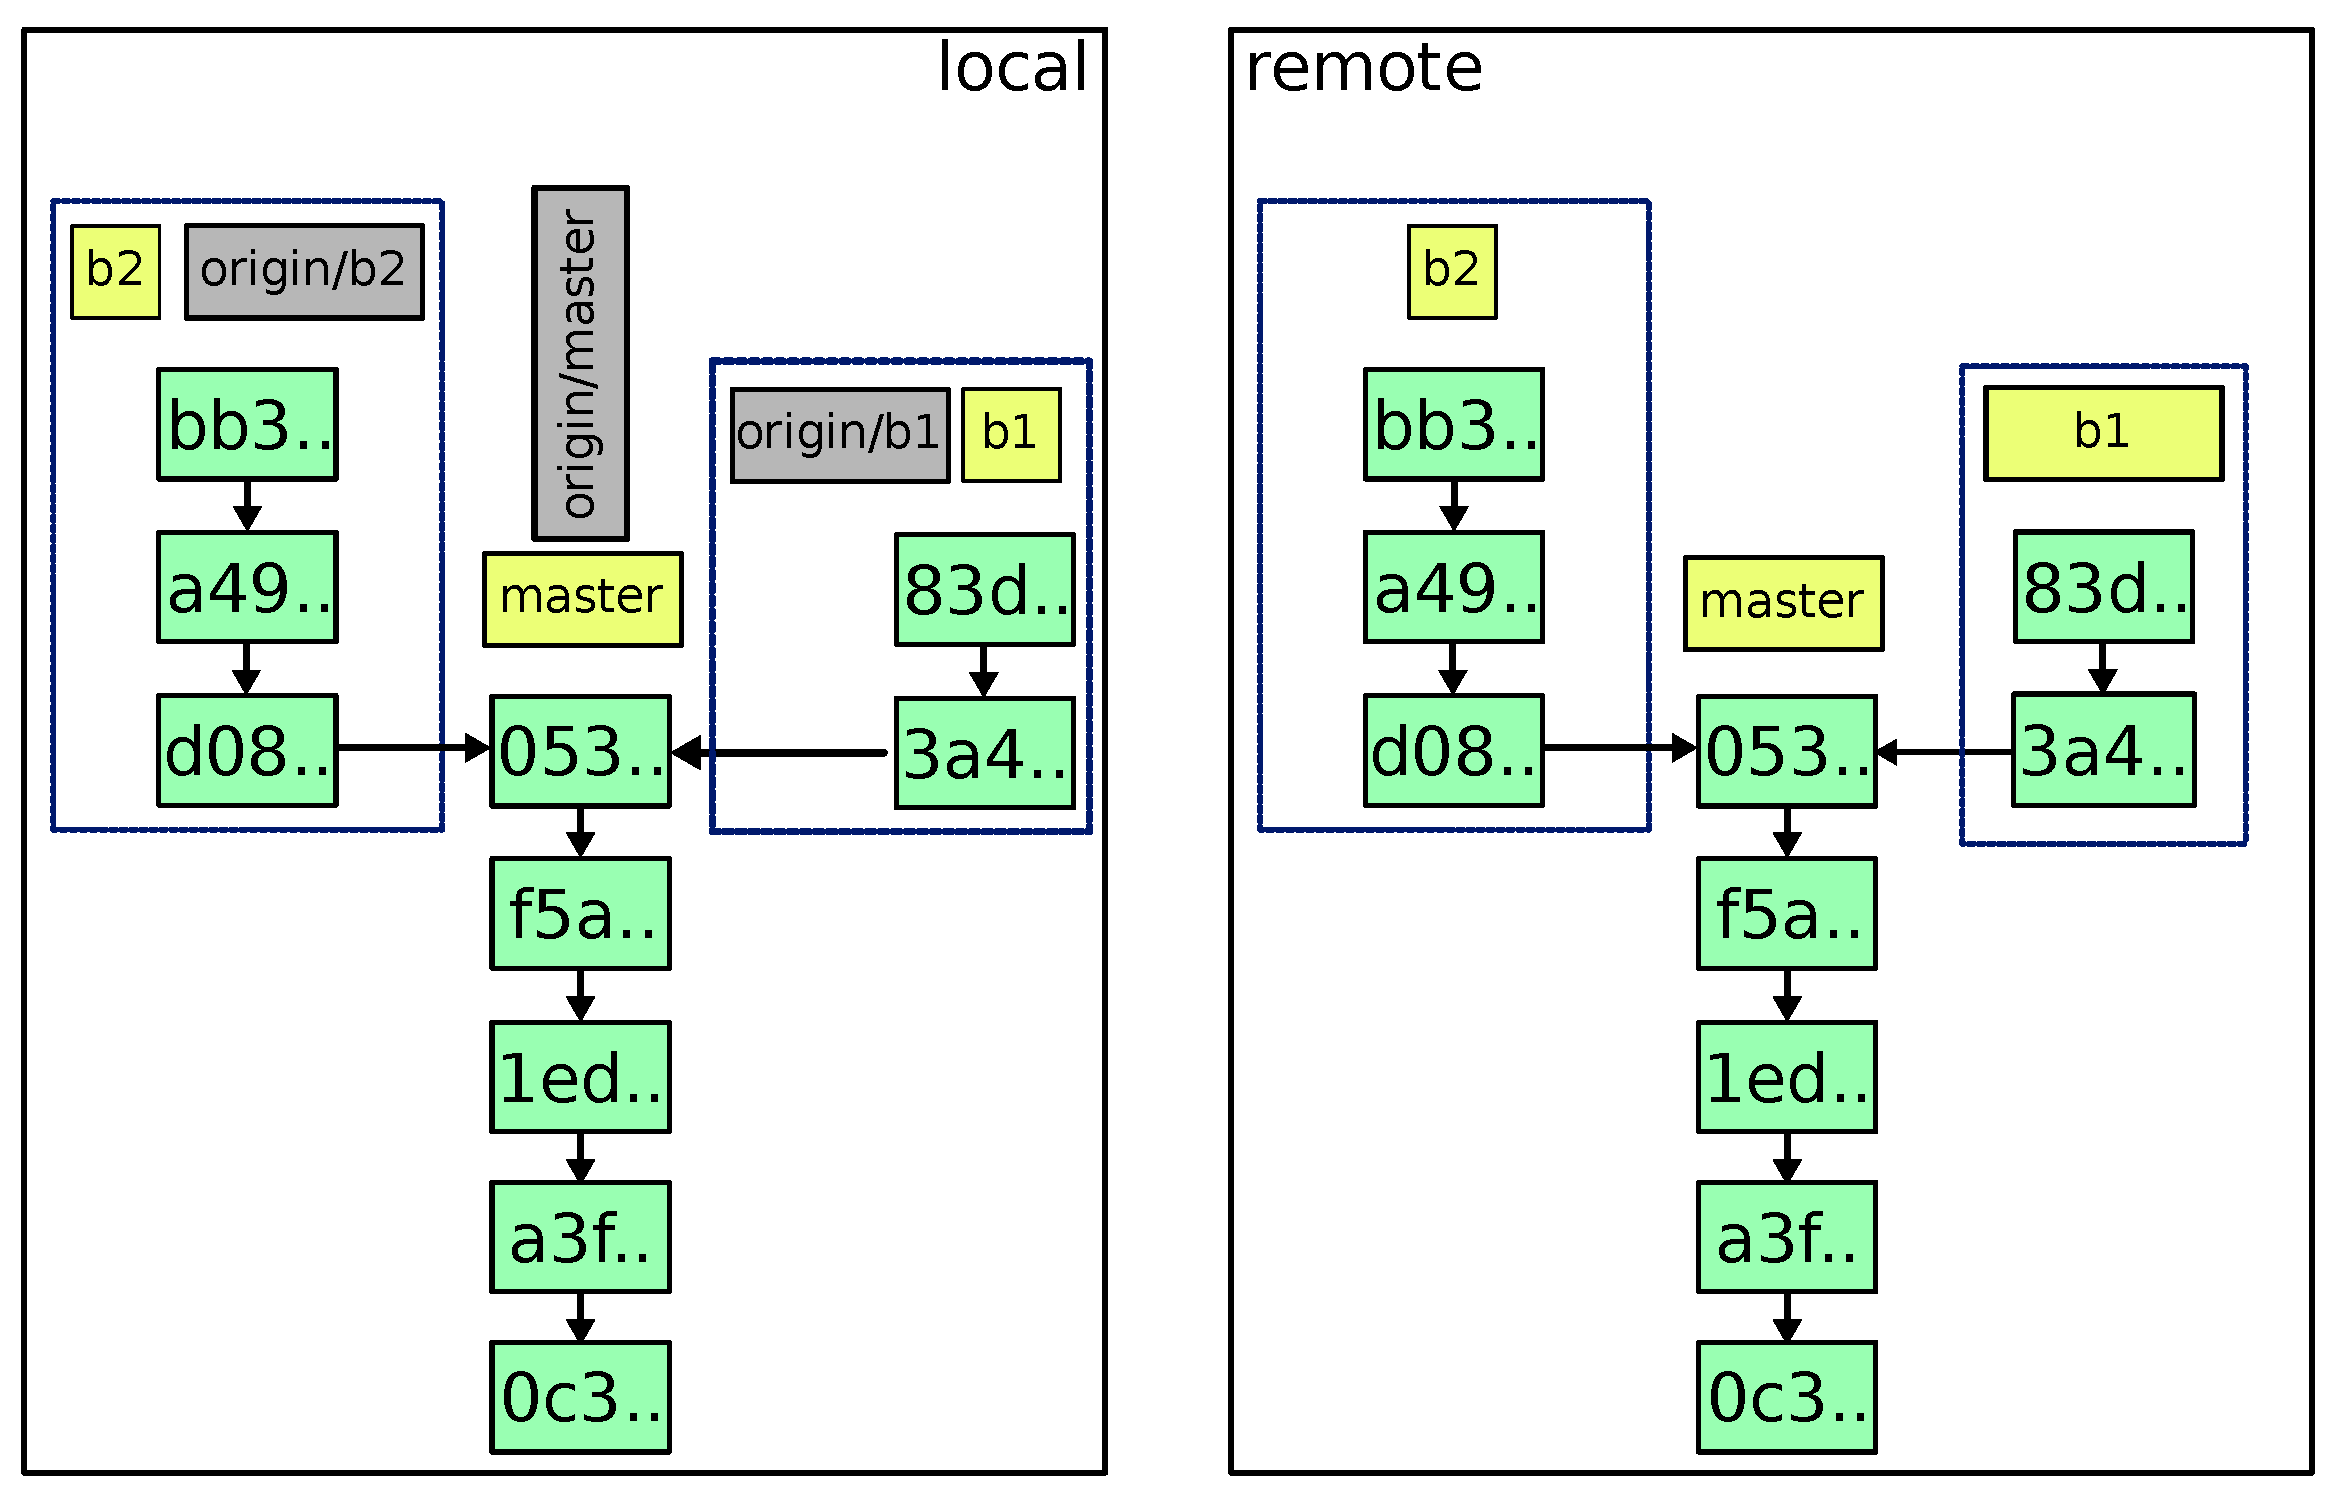
\includegraphics[width=\textwidth]{img/6.pdf}
\end{frame}

\begin{frame}{}
  \begin{itemize}
  \item \lstinline|git push origin b1:master|
  \end{itemize}
\end{frame}

\begin{frame}{}
  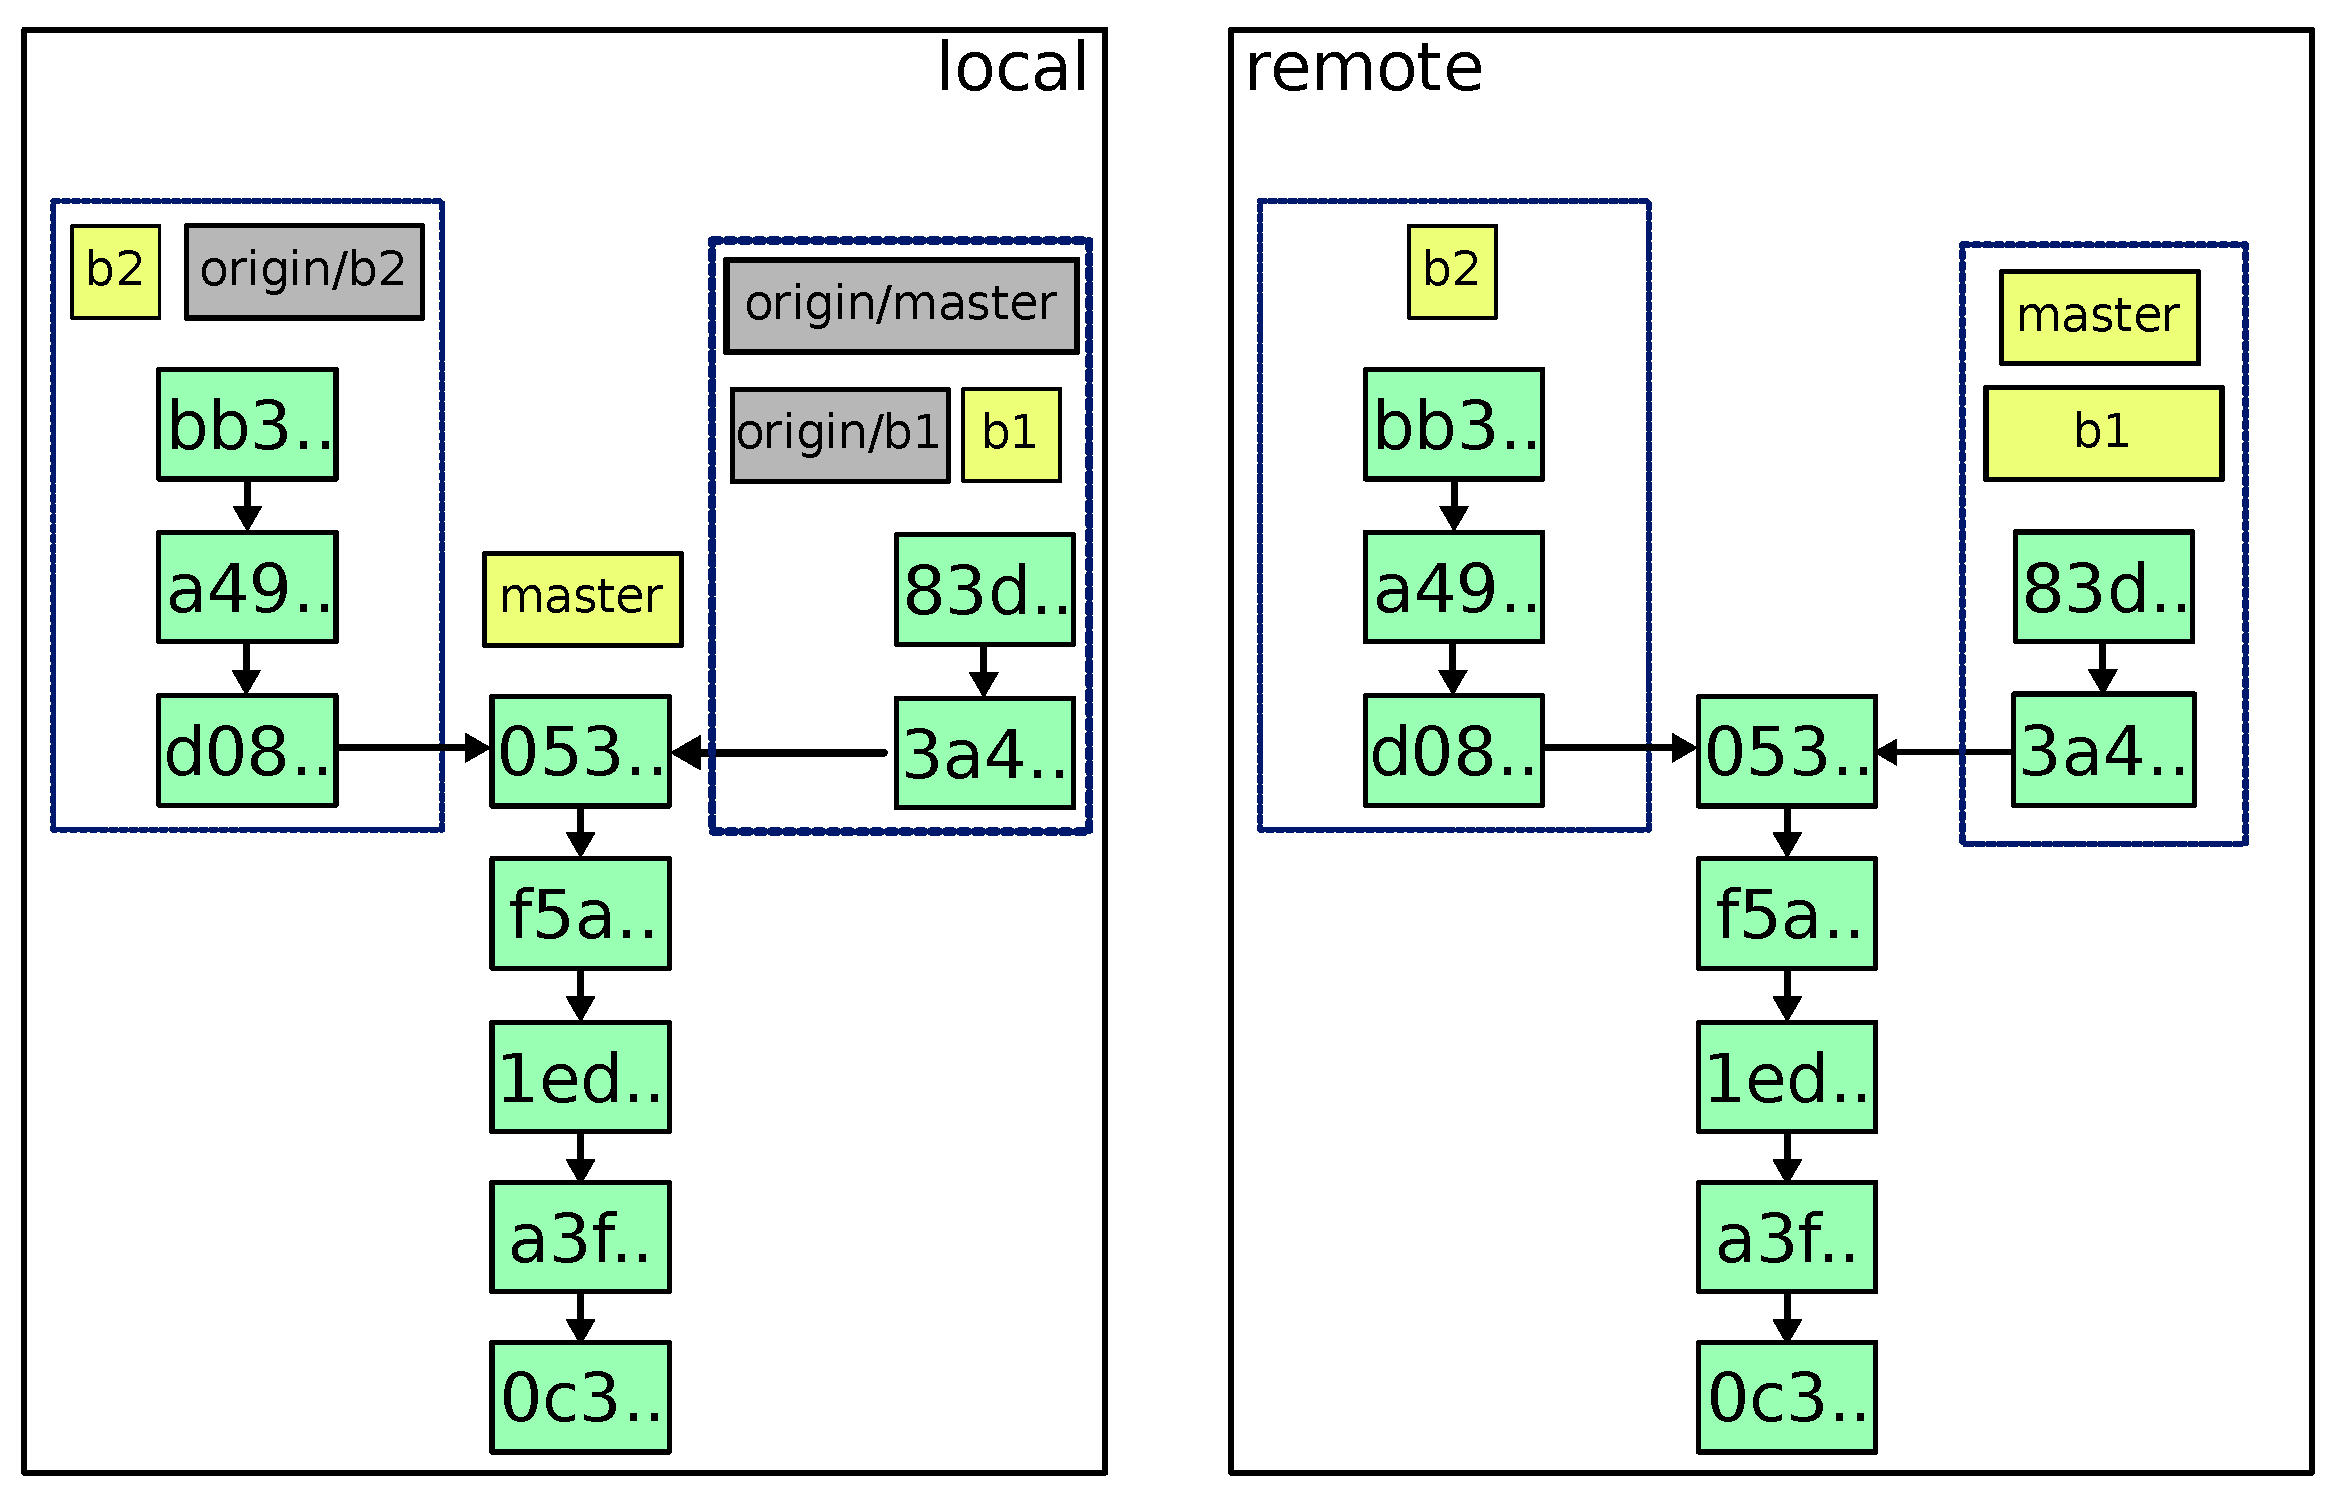
\includegraphics[width=\textwidth]{img/7.pdf}
\end{frame}

\begin{frame}{}
  \begin{itemize}
  \item \lstinline|git pull origin master|
  \item \lstinline|git branch -D b2|
  \item \lstinline|git push origin :b2|
  \end{itemize}
\end{frame}

\begin{frame}{}
  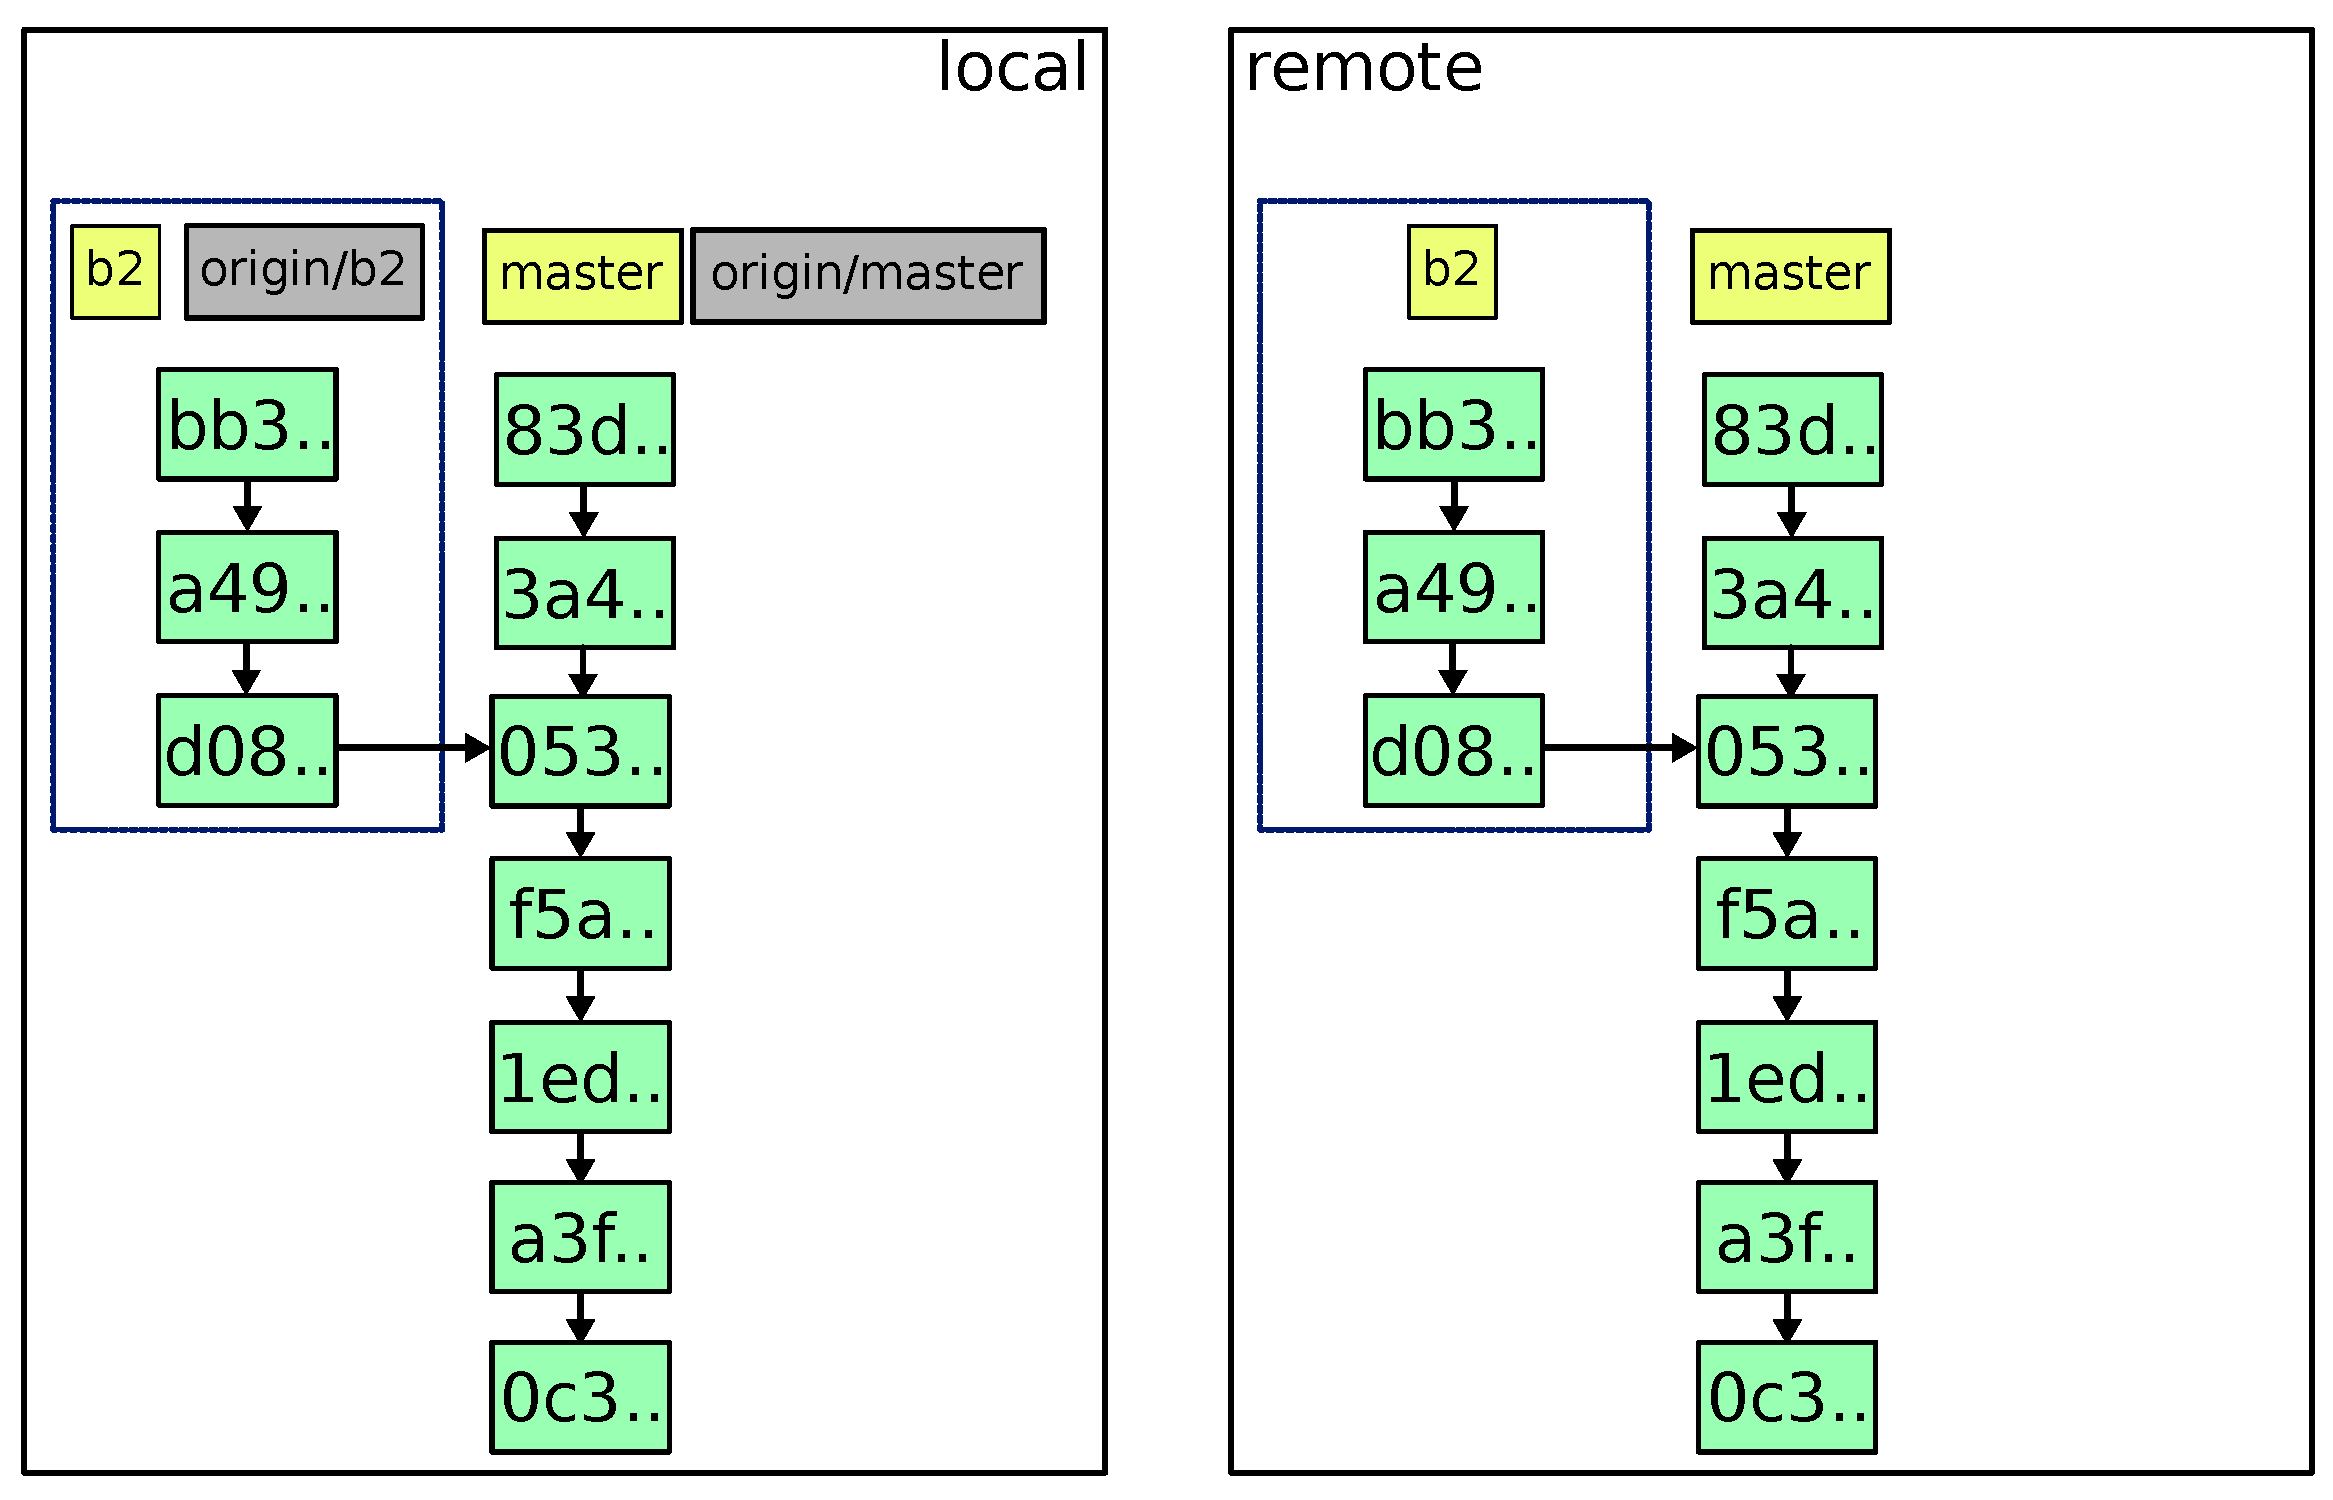
\includegraphics[width=\textwidth]{img/8.pdf}
\end{frame}

\begin{frame}{}
  \begin{itemize}
  \item \lstinline|git rebase master b2|
  \item \lstinline|git push origin b2|
  \end{itemize}
\end{frame}

\begin{frame}{}
  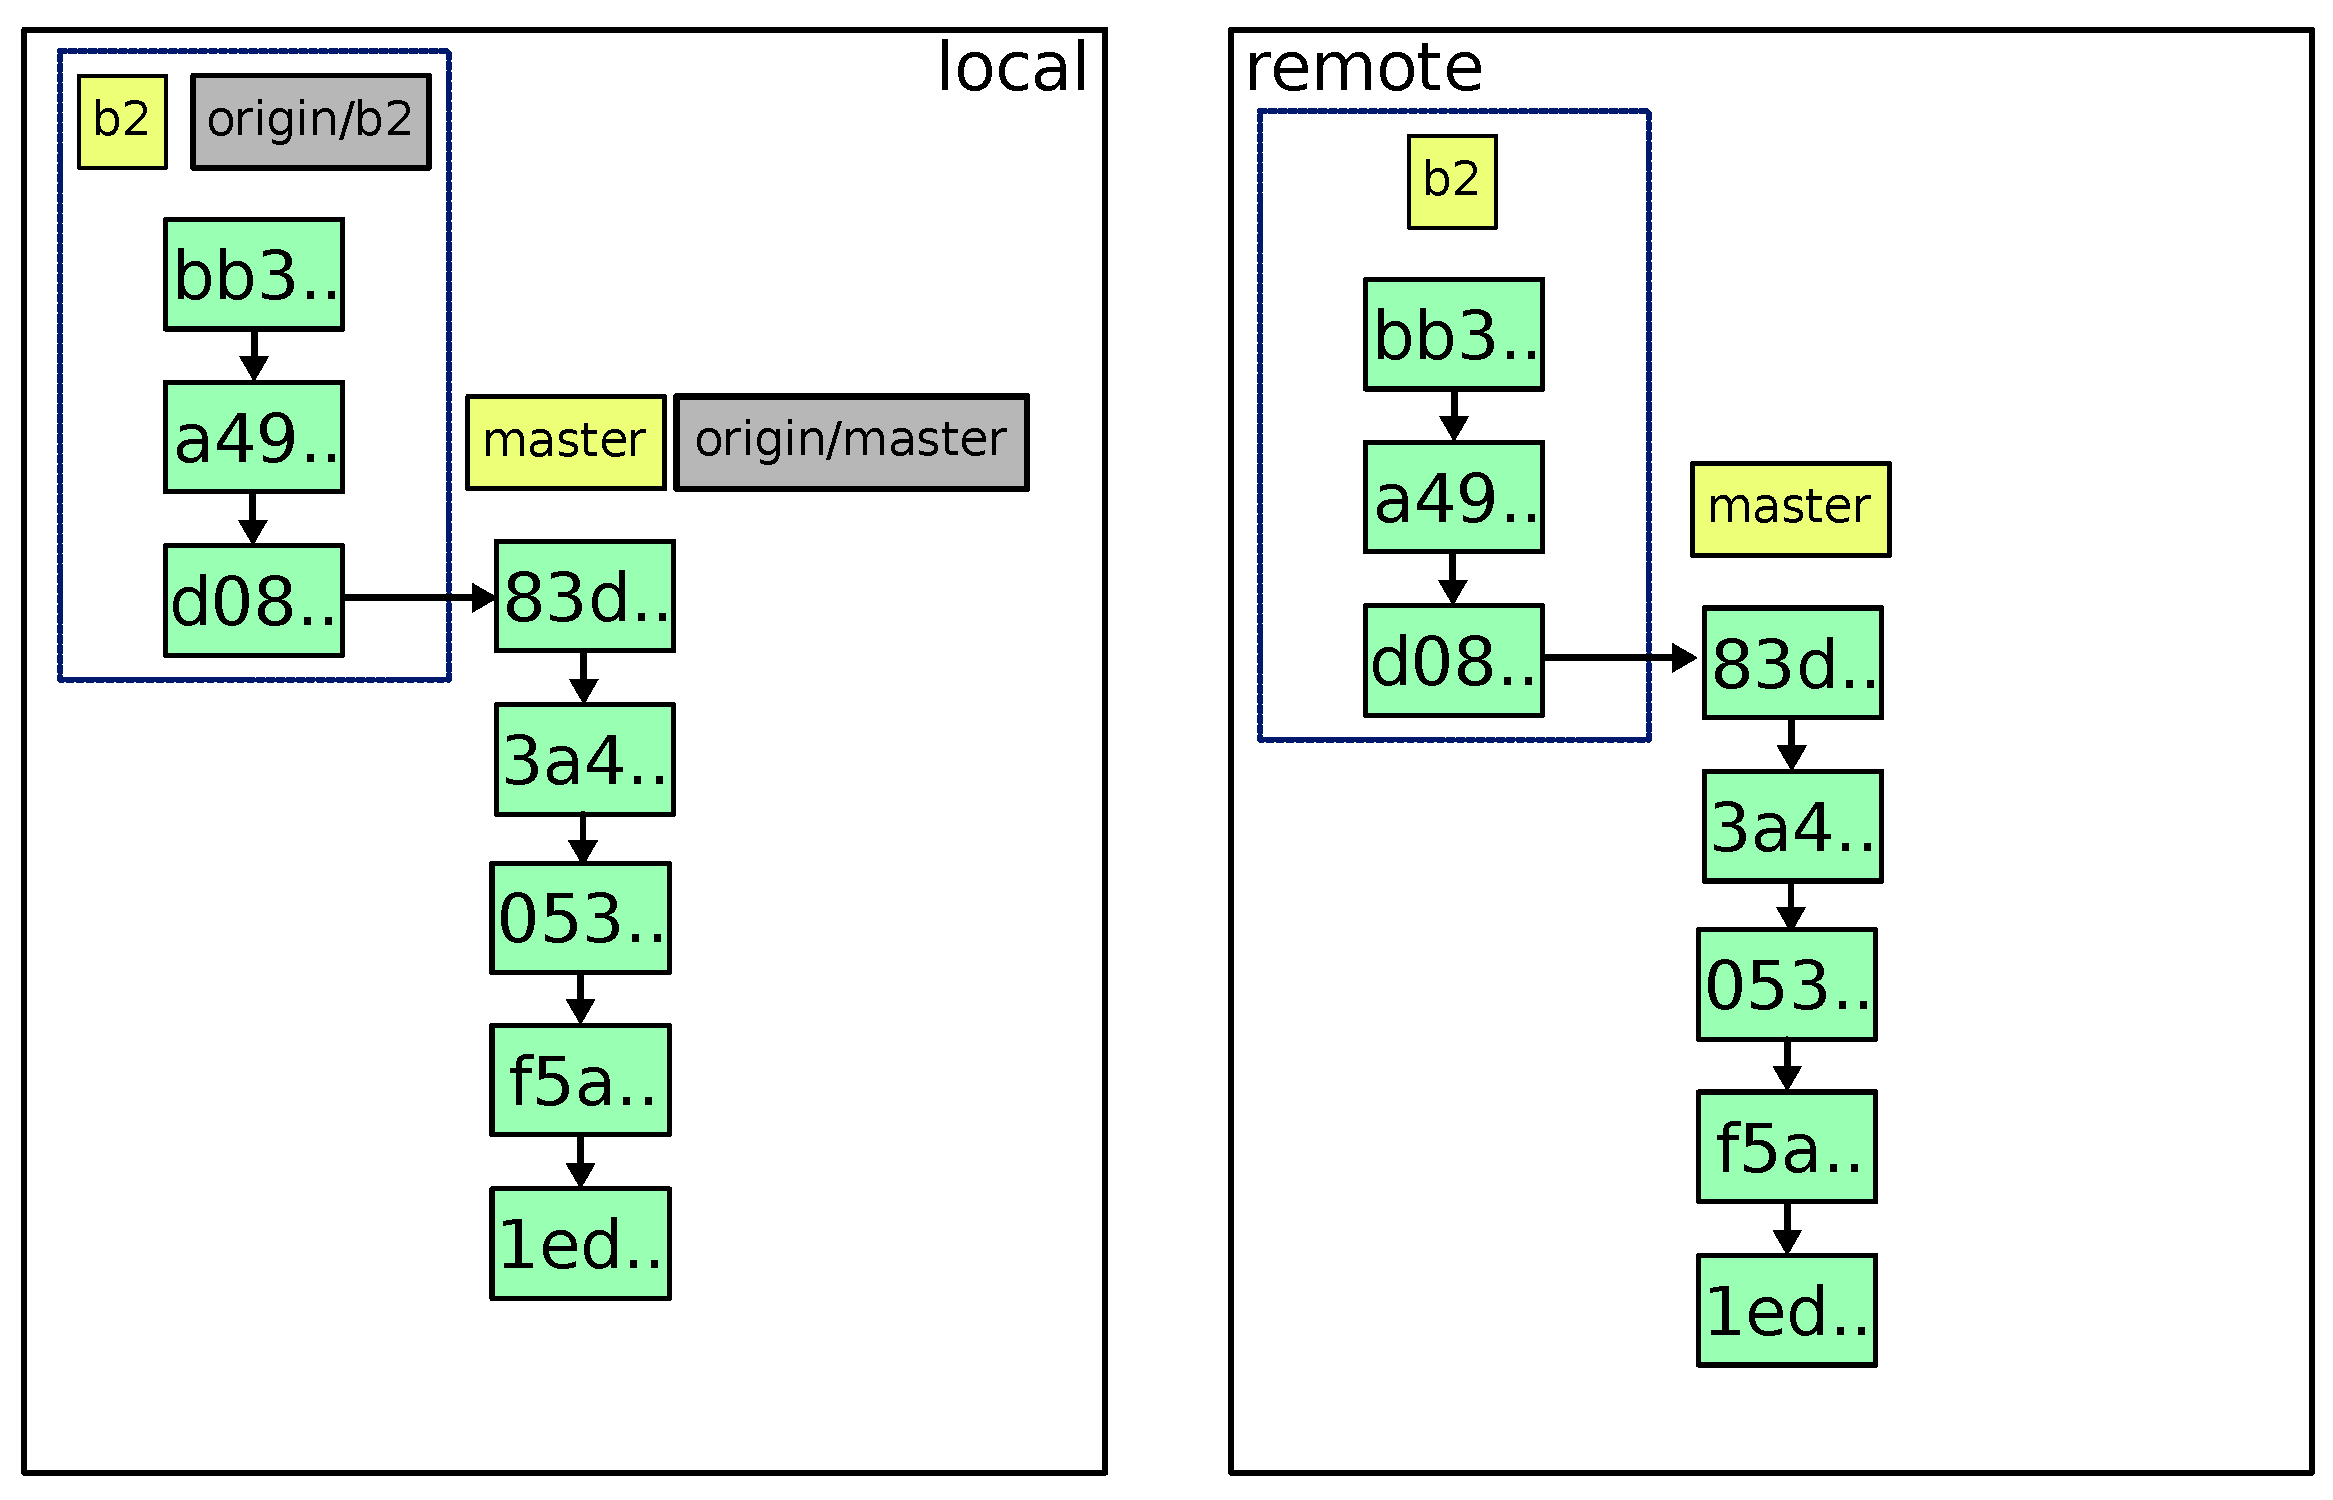
\includegraphics[width=\textwidth]{img/9.pdf}
\end{frame}

\begin{frame}{}
  \begin{itemize}
  \item \lstinline|git push origin b2:master|
  \item \lstinline|git branch -D b2|
  \item \lstinline|git push origin :b2|
  \item \lstinline|git pull origin master|
  \end{itemize}
\end{frame}

\begin{frame}{}
  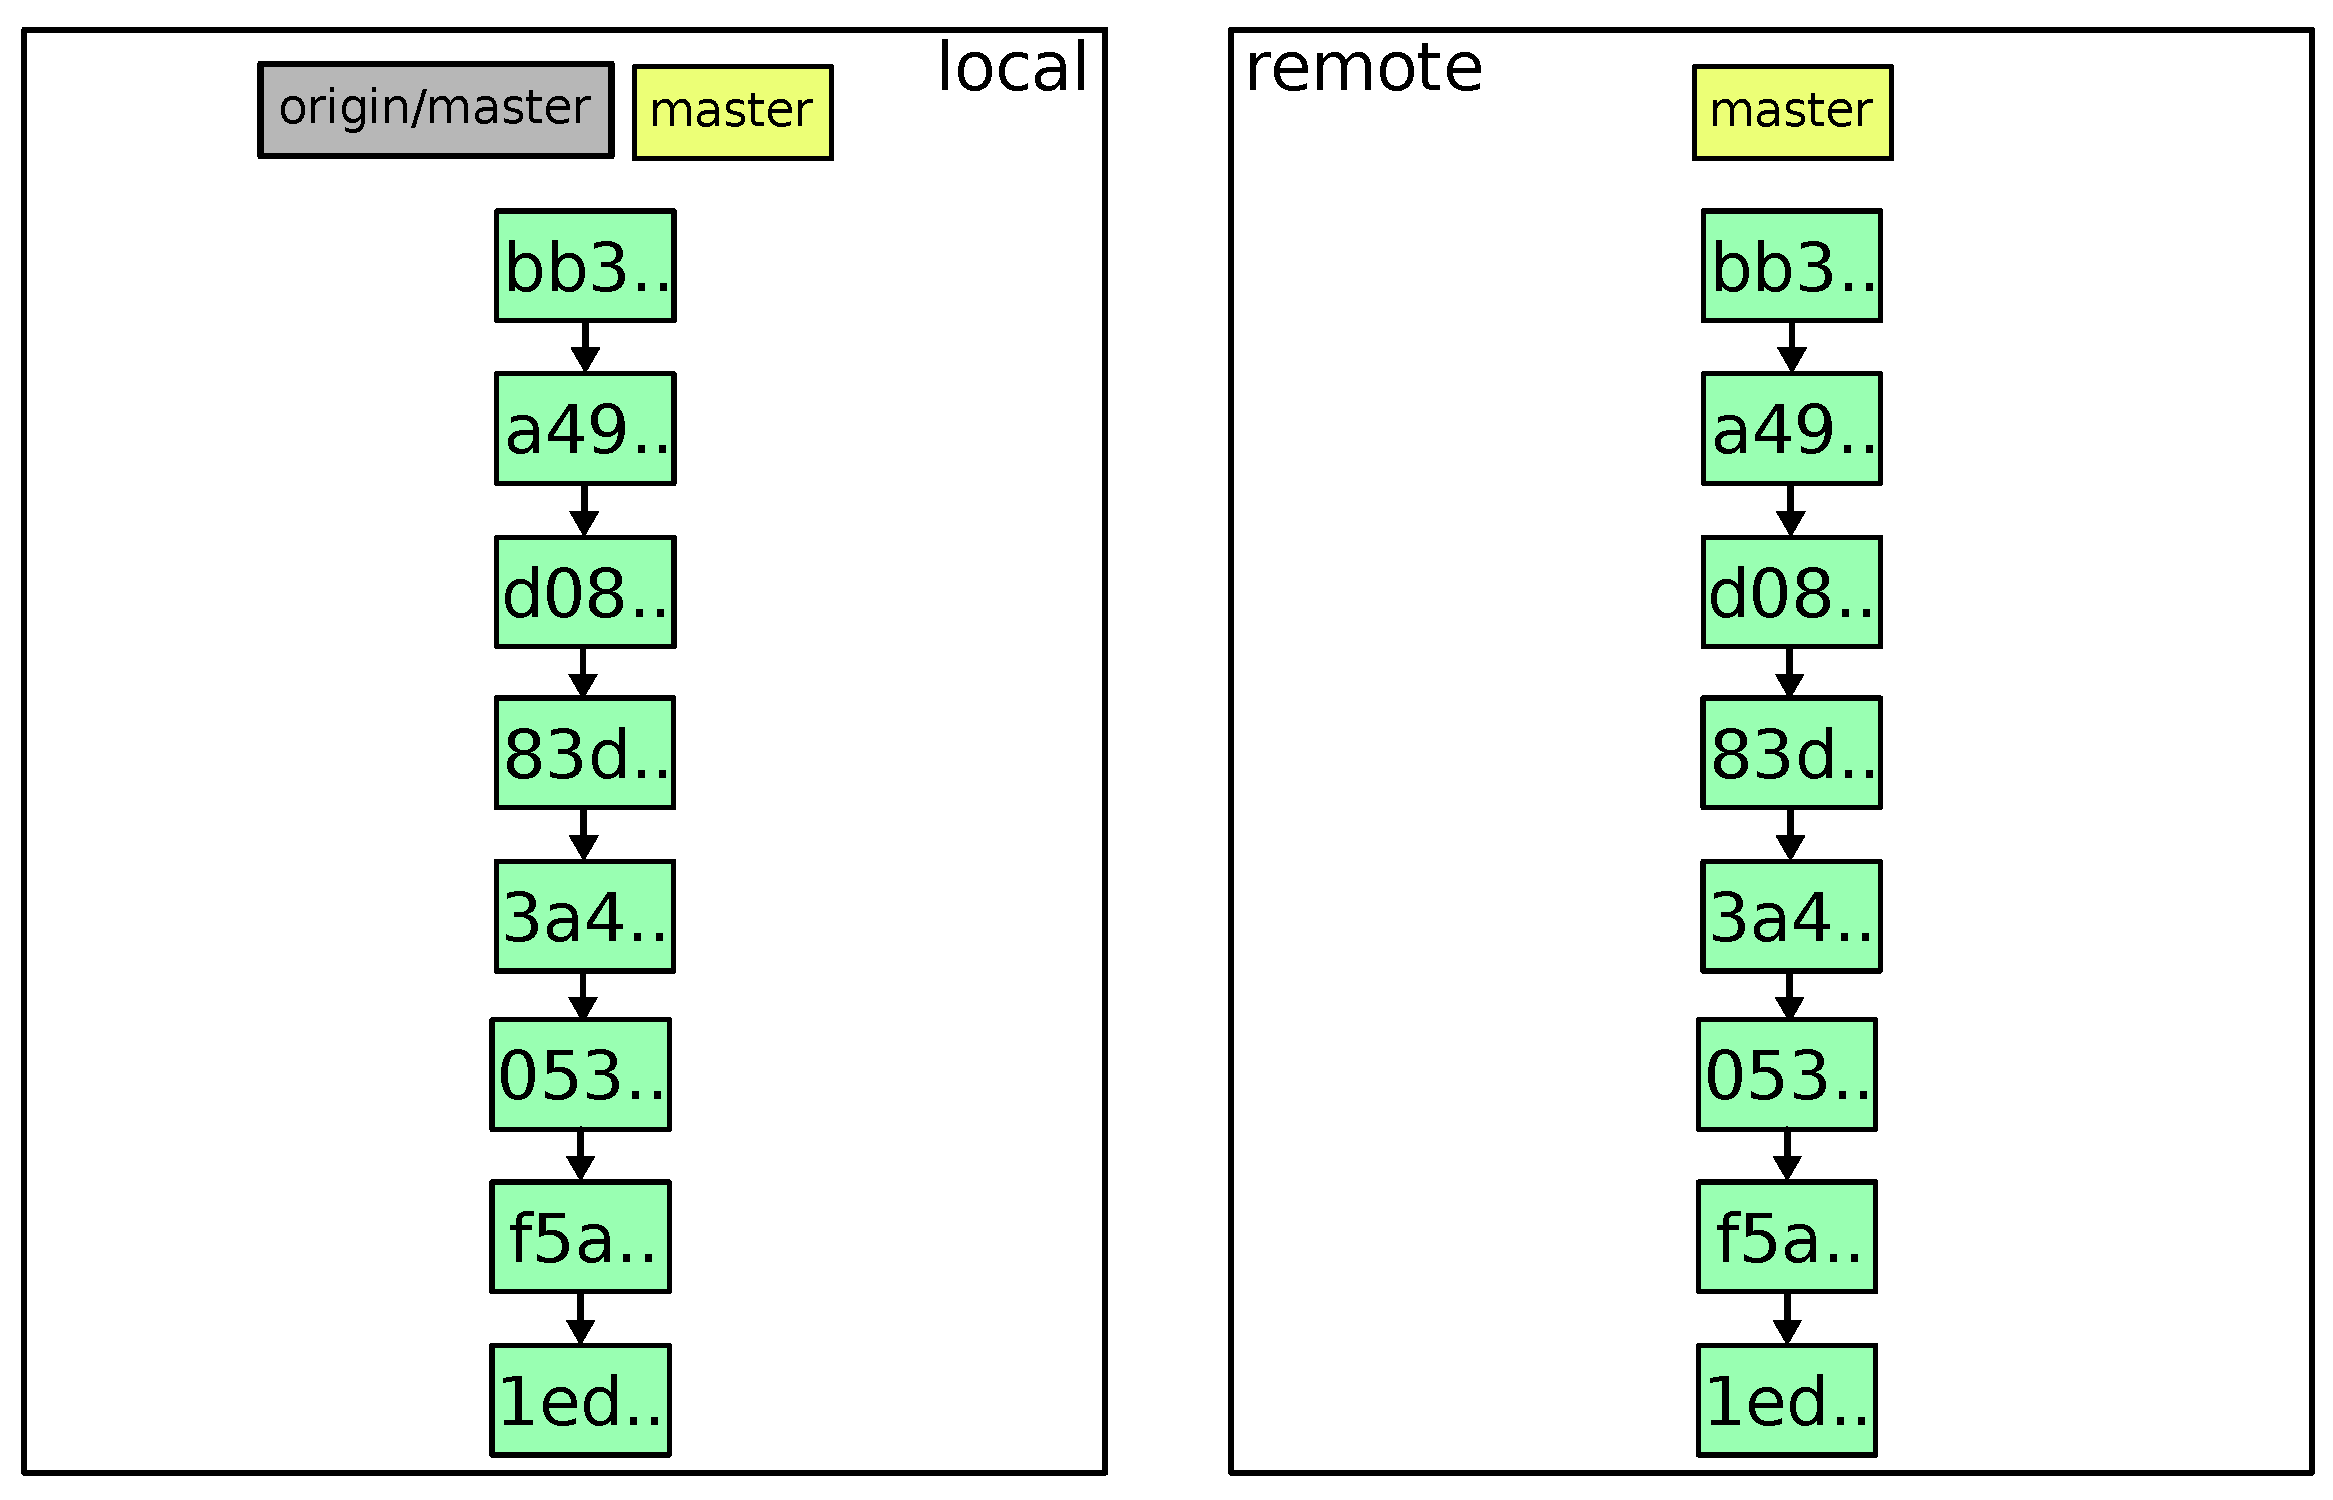
\includegraphics[width=\textwidth]{img/10.pdf}
\end{frame}

\begin{frame}{}
  \begin{center}
  \Huge \dots
  \end{center}
\end{frame}

%------------------------------------------------------------

\section{Ressources}
\begin{frame}{Ressources}
  \begin{itemize}
  \item \href{http://progit.org/about.html}{Progit}
  \item \href{http://git.or.cz/gitwiki/GitHosting}{Liste de serveurs \git}
  \end{itemize}
\end{frame}

\end{document}
